\documentclass[a4paper,11pt,twoside]{memoir}
\setcounter{secnumdepth}{2}
\let\STARTCODE\relax 
\let\STOPCODE\relax 
\STARTCODE
\usepackage{color,calc,graphicx,soul}
\definecolor{nicered}{rgb}{.647,.129,.149} \makeatletter
\newlength\dlf@normtxtw \setlength\dlf@normtxtw{\textwidth}
\def\myhelvetfont{\def\sfdefault{mdput}} \newsavebox{\feline@chapter}
\newcommand\feline@chapter@marker[1][4cm]{
  \sbox\feline@chapter{
    \resizebox{!}{#1}{\fboxsep=1pt
      \colorbox{nicered}{\color{white}\bfseries\sffamily\thechapter}
    }}
  \rotatebox{90}{
    \resizebox{
      \heightof{\usebox{\feline@chapter}}+\depthof{\usebox{\feline@chapter}}}
    {!}{\scshape\so\@chapapp}}\quad
  \raisebox{\depthof{\usebox{\feline@chapter}}}{\usebox{\feline@chapter}}
} \newcommand\feline@chm[1][4cm]{
  \sbox\feline@chapter{\feline@chapter@marker[#1]}
  \makebox[0pt][l]{
    \makebox[1cm][r]{\usebox\feline@chapter}
  }} \makechapterstyle{daleif1}{
  \setlength{\afterchapskip}{10pt}
  \renewcommand{\insertchapterspace}{}
  \renewcommand\chapnamefont{\normalfont\Large\scshape\raggedleft\so}
  \renewcommand\chaptitlefont{\normalfont\huge\bfseries\scshape\color{nicered}}
  \renewcommand\chapternamenum{} 
  \renewcommand\printchaptername{}
  \renewcommand\printchapternum{\vspace{-1.8cm}\null\hfill\feline@chm[2.5cm]\par}
  \renewcommand\afterchapternum{\par\vskip\midchapskip}
  \renewcommand\printchaptertitle[1]{\chaptitlefont\raggedleft
  	##1\par}
  \renewcommand\printchapternonum{\vspace{0.2cm}}
}

\makeatother
\chapterstyle{daleif1}
\STOPCODE
\usepackage[utf8x]{inputenc}
\usepackage[T1]{fontenc}
\usepackage[english, french]{babel}
\usepackage{lipsum}
\usepackage{lmodern}
\rmfamily
\DeclareFontShape{T1}{lmr}{b}{sc}{<->ssub*cmr/bx/sc}{}
\DeclareFontShape{T1}{lmr}{bx}{sc}{<->ssub*cmr/bx/sc}{}
\usepackage{epigraph}
\usepackage[french]{minitoc}
\setcounter{minitocdepth}{2}
\usepackage{soul}
\usepackage[pagebackref,colorlinks=true,citecolor=forestgreen,linkcolor=black,menucolor=alezan,urlcolor=prune]{hyperref}
\renewcommand*{\backref}[1]{}
\renewcommand*{\backrefalt}[4]{
\ifcase #1
-- Non cité.
\or
-- Cité page~#2.
\else
-- Cité pages~#2.
\fi}
\renewcommand*{\backrefsep}{, }
\renewcommand*{\backreftwosep}{ et~}
\renewcommand*{\backreflastsep}{ et~}
\usepackage{lingmacros}
\usepackage{fancybox}
\usepackage{pifont}
\usepackage{dsfont}
\def\sep{\begin{center}\begin{large}\ding{167}\end{large}\end{center}}
\renewcommand{\bibname}{Bibliographie}
\addto{\captionsenglish}{\renewcommand{\bibname}{Bibliographie}}
\addto{\captionsfrench}{\renewcommand{\listfigurename}{Liste des figures}}
\usepackage{newcent}
\usepackage{helvet}
\usepackage{color}
\usepackage{colortbl}
\usepackage{multirow}
\usepackage{longtable}
\newcommand{\withnofdp}[1]{{\NoAutoSpaceBeforeFDP #1}}
\usepackage{arydshln}
\usepackage{listings}
\lstset{
  language=XML, 
  basicstyle=\small,
  showspaces=false,
  showstringspaces=false,
  breaklines=true,
  breakatwhitespace=true,
  morecomment=[s]{<!--}{-->},
  alsoletter=.-,
  commentstyle=\itshape\color{gray},
  markfirstintag=true,
  string=[d]",
  keywords={correction},
  keywordstyle=\color{alizarine},
  stringstyle=\color{acier},
}
\usepackage{pgf,pgfarrows,pgfnodes}
\usepackage{tikz}
\usepackage{tikz-qtree}
\usepackage{tikz-dependency}
\usepackage{pgfplots}
\usetikzlibrary{mindmap,trees, backgrounds}
\usepackage{filecontents}
\usepackage{qtree}
\definecolor{acier}{HTML}{3A8EBA}
\definecolor{alezan}{HTML}{A76726}
\definecolor{alizarine}{HTML}{D90115}
\definecolor{amande}{HTML}{82C46C}
\definecolor{ambre}{HTML}{F0C300}
\definecolor{abricot}{HTML}{E67E30}
\definecolor{grey}{rgb}{0.9,0.9,0.9}
\definecolor{gris}{rgb}{0.1,0.1,0.1}
\definecolor{forestgreen}{rgb}{0.13,0.54,0.13}
\definecolor{dockerblue}{rgb}{0.11,0.56,0.98}
\definecolor{orange}{rgb}{0.64,0.16,0.16}
\definecolor{ocre}{HTML}{DFAF2C}
\definecolor{prune}{HTML}{811453}
\newcommand{\remCyril}[1]{\textcolor{dockerblue}{\emph{CG : #1}}}
\newcommand{\myex}[1]{\color{acier}{\emph{#1}}\color{black}}
\newcommand{\rg}[1]{\textsl{Remarque : #1}}
\def\euro{\mbox{\raisebox{.25ex}{{\it =}}\hspace{-.5em}{\sf C}}}
\newenvironment{changemargin}[2]{\begin{list}{}{
\setlength{\topsep}{0pt}
\setlength{\leftmargin}{0pt}
\setlength{\rightmargin}{0pt}
\setlength{\listparindent}{\parindent}
\setlength{\itemindent}{\parindent}
\setlength{\parsep}{0pt plus 1pt}
\addtolength{\leftmargin}{#1}
\addtolength{\rightmargin}{#2}
}\item }{\end{list}}
\usepackage{chngpage}
\usepackage{amssymb,amsmath,amsthm,amscd}
\usepackage{mathrsfs}
\usepackage{subfig}
\usepackage{tabularx}
\usepackage{calc}
\usepackage{graphicx}
\usepackage{hyperref}
\usepackage{makeidx}

% Numérotation des lignes
%\usepackage{lineno}
%\linenumbers

% comments in margin with \todo command
\usepackage[colorinlistoftodos]{todonotes} % option disable to hide todos
% command todo : options
% - noline: no line connecting the note with the place in the text
%   where the note occurs in the latex code
% - fancyline : curved arrow from note to inssertion point
% - inline: place a todonote inside the text instead of in the margin
% - author=name
\newcommand{\florent}[1]{\todo[noline,size=\tiny,color=yellow!40]{#1}}
%\renewcommand{\florent}[1]{} % uncomment for final

\makeindex
\usepackage[french,intoc,refpage]{nomencl}
\renewcommand{\nomname}{Glossaire}
\renewcommand*{\pagedeclaration}[1]{\unskip\dotfill\hyperpage{#1}}
\makenomenclature
\newcommand{\nocontentsline}[3]{}
\newcommand{\tocless}[2]{\bgroup\let\addcontentsline=\nocontentsline#1{#2}\egroup}
%%%%%%%%%%%%%%%%%%%%%%%%%%%%%%%%%%%%%%%%%%%%%%%%%%%%%%%
%% EN-TETES ET PIEDS DE PAGE
\let\footruleskip\undefined
\usepackage{fancyhdr}
\pagestyle{fancy} % Activer le style de pages personnalisé
\fancyhf{} % Remettre à zéro des en-tête et pied de page
\setlength{\headheight}{14pt} % Fixer la hauteur de l'espace réservé à l'en-tête du haut

%%% Pas de numéro de page sur la première page des chapitres
\makeatletter
\let\ps@plain=\ps@empty
\makeatother

%===================== Style 1 =================================================
\fancyhead[RO,LE]{
\thepage
}
\fancyhead[LO]{\scshape \nouppercase{\rightmark}}
\fancyhead[RE]{\scshape \nouppercase{\leftmark}} 
\renewcommand{\headrulewidth}{.4pt}
\fancyfoot{}

%================================== Style 2 ====================================
\let\origdoublepage\cleardoublepage
\newcommand{\clearemptydoublepage}{
  \clearpage
  {\pagestyle{empty}\origdoublepage}
}
\let\cleardoublepage\clearemptydoublepage
\FrenchFootnotes
\AddThinSpaceBeforeFootnotes

%%%%%%%%%%%%%%%%%%%%%%%%%%%%%%%%%%%%%%%%%%%%%%%%%%%%%%%

\newcommand*\chapterstar[1]{
  \chapter*{#1}
  \addcontentsline{toc}{chapter}{#1}
  \markboth{#1}{#1}}


%%%%%%%%%%%%%%%%%%%%%%%%%%%%%%%%%%%%%%%%%%%%%%%%%%%%%%%
% ENVIRONNEMENTS DE THEOREMES
\theoremstyle{plain} % style plain
\newtheorem{theo}{Théorème}[chapter]
\newtheorem{cor}[theo]{Corollaire}
\newtheorem{prop}[theo]{Proposition}
\newtheorem{lem}[theo]{Lemme}
\newtheorem{conj}[theo]{Conjecture}
\newtheorem*{theoetoile}{Théorème} % théorème non numéroté
\newtheorem*{conjetoile}{Conjecture} % conjecture non numérotée

\theoremstyle{definition} % style definition
\newtheorem{defi}[theo]{Définition}
\newtheorem{exemple}[theo]{Exemple}
\newtheorem{question}[theo]{Question}
\newtheorem{remarque}[theo]{Remarque}
\newtheorem{notation}[theo]{Notation}

% Pour renommer ``preuve'' en ``démonstration''
\renewcommand{\proofname}{Démonstration}


%%%%%%%%%%%%%%%%%%%%%%%%%%%%%%%%%%%%%%%%%%%%%%%%%%%%%%%
% ENVIRONNEMENTS DEDICACE ET EPIGRAPHE
\newenvironment{dedicace}{%
  \newpage\thispagestyle{empty}e
  \hfill\begin{minipage}{100mm}\begin{flushright}\it}{%
  \end{flushright}\end{minipage}\vfill}

\newenvironment{epigraphe}{%
  \hfill\begin{minipage}{60mm}\begin{flushright}\footnotesize\it}{%
  \end{flushright}\end{minipage}\hspace*{7mm}\vfill}

\newcommand\tab[1][5mm]{\hspace*{#1}}
\parindent=0em
\begin{document}
\sloppy
\dominitoc
% ================================ Page du garde ==============================

\pdfbookmark[0]{Page de garde}{garde}
\thispagestyle{empty}

\begin{center}
  \begin{tabularx}{\textwidth}{m{10.3cm}m{4cm}}
	 
\includegraphics[width = 3.9cm]{z_images/0_logos/0_inalco.png} %% CG : 3.5cm au lieu de 3 cm
	&
        %% TODO: remplacer le logo du LIMSI par celui de la société ou
        %% du laboratoire où vous avez réalisé votre stage (si le
        %% sujet du mémoire de recherche fait suite à votre stage)
	 
\includegraphics[width = 3.9cm]{z_images/0_logos/1_inria.png} %% CG : 3.5cm au lieu de 3 cm
        \\ \hline
  \end{tabularx}
\end{center}

\begin{center}
\vspace{\stretch{1}}
% Permet de créer un espace vertical de longueur variable (\stretch) et de "poids" 1
{\Large \textbf{Institut National des Langues et Civilisations Orientales}}

\vspace{\stretch{1}}

{\normalsize Département Textes, Informatique, Multilinguisme}

\vspace{\stretch{2}}
\hrule
\vspace{\stretch{1}}
%% TODO: indiquez le titre de votre mémoire
{\LARGE \textbf{Titre du mémoire}}
\vspace{\stretch{1}}
\hrule

\vspace{\stretch{2}}

{\Huge \textsc{Master}}

\vspace{\stretch{1}}

{\LARGE \textsc{Traitement Automatique des Langues}}

\vspace{\stretch{1}}

{\normalsize \emph{Parcours~:}}

\vspace{\stretch{0.5}}

%% TODO: indiquez votre parcours
{\normalsize \emph{Ingénierie Multilingue}}

\vspace{\stretch{1}}

{\large par}

\vspace{\stretch{1}}

%% TODO: indiquez vos nom et prénom
\textbf{{\LARGE Martin \textsc{DIGARD}}}

\vspace{\stretch{2}}

{\normalsize \emph{Directeur de mémoire~:}}

\vspace{\stretch{0.5}}

%% TODO: indiquez le nom du/des directeur(s) de mémoire (enseignant
%% INaLCO qui supervise votre travail)
{\normalsize \emph{Damien NOUVEL}}

\vspace{\stretch{2}}

{\normalsize \emph{Encadrant~:}}

\vspace{\stretch{0.5}}

%% TODO: indiquez le nom du/des encadrant(s) de stage si votre mémoire
%% porte sur votre travail de stage
{\normalsize \emph{Florent JACQUEMARD}}

\vspace{\stretch{2}}

{\normalsize Année universitaire 2020-2021}

\end{center}

\cleardoublepage % pour laisser une page blanche au verso de la page de garde

\newpage
\setcounter{tocdepth}{1}
\pdfbookmark[0]{Table des matières}{tablematieres}
\tocless\tableofcontents
\newpage
\listoffigures
\listoftables
\printnomenclature
\newpage
%%%%%%%%%%%%%%%%%%%%%%%%%%%%%%%%%%%%%%%%%%%%%%%%%%%%%%%%%%%%%%%%%%%%%%%%%%%%%%%%%%


\chapter*{Introduction générale}
\adjustmtc
\addstarredchapter{Introduction générale} 
% !TEX root = 1_memoire.tex
Ce mémoire de recherche, effectué en parallèle d’un stage à l’Inria dans le
cadre du master de traitement automatique des langues de l’Inalco, contient
une proposition originale ainsi que diverses contributions ayant toutes pour
\florent{"ayant toutes pour objectif..." $\to$ dans le domaine de la transcription musicale automatique 
objectif d’améliorer \textbf{qparse}, un outil de transcription automatique de
et plus spécifiquement, dans le cas de la batterie.}
la musique sur sa capacité à transcrire la batterie. 
Nous ne parlerons donc pas
\florent{transcription musicale, suivant des méthodes communes/issues du TAL (éviter les négations)}
directement de langues naturelles, mais de l’écriture
\florent{"l’écriture" $\to$ la génération}
automatique de partitions
de musique à partir de données audio ou symboliques. La musique et les langues
naturelles sont deux moyens que nous servent à exprimer nos ressentis sur le
monde et les choses : « La musique s’écrit et se lit aussi facilement qu’on lit
et écrit les paroles que nous prononçons. » \cite{danhauser}.
Cet exercice nécessite la manipulation d’un langage
musical codifié par une grammaire (solfège, durées, nuances, volumes) et
soulèvera des problématiques concernées par les techniques du traitement
automatique des langues.

L’écriture musicale offre de nombreuses possibilités pour la transcription d’un
rythme donné. Le contexte musical ainsi que la lisibilité d’une partition pour
un batteur entraîné conditionnent les choix d’écriture. Reconnaître la
métrique principale d’un rythme, la façon de regrouper les notes par les
ligatures, ou simplement décider d’un usage pour une durée parmi les
différentes continuations possibles (notes pointées, liaisons, silences, etc.)
constituent autant de possibilités que de difficultés.

\florent{il faut revoir la fin, avec une description rapide du problème, 
         de la méthode suivie et des contributions} %suivi d'un petit plan par parties.
Voici la proposition de ce mémoire ainsi que les contributions apportées lors
du stage :
Rédiger entièrement la liste à puce qui suit.
\begin{itemize}
	\item Proposition principale : les systèmes (\ref{systemes_methodes},
		\ref{expe_theo}) :\\
	Recherche de rythmes génériques en amont dans la chaîne de traitement.\\
	$\Rightarrow$ L’objectif de fixer des choix le plus tôt possible afin de
	simplifier le reste des calculs en éliminant une partie d’entre eux. Ces
	choix concernent notamment la métrique et les règles de réécriture.
	\item Une description de la notation de la batterie
		(\ref{notation_batterie})
	\item Une modélisation de la transcription de la batterie
		(\ref{modelisation_transcription})
	\item Analyse MIDI-Audio (\ref{analyse_midi_audio})
	\item Transcription manuelle de partition \ref{partition_entiere}
	\item Expérimentation théorique d’un système \ref{expe_theo}
	\item Théorie et tests unitaires pour le passage au polyphonique
		(\ref{jam_tests})
	\item Création de grammaires pondérées pour la batterie (\ref{gram_pond})
	\item Contributions sur la branche « distance » dans :
	\begin{itemize}
		\item qparselib/notes/cluster.md
		\item qparselib/src/segment/import/ :\\
		DrumCode hpp et cpp\\
	\end{itemize}
\end{itemize}

Au lieu du paragraphe final : Nous présenterons dans un premier temps les
parallèles entre TAL et MIR, puis les spécificités de la notation pour la
batterie……… 

\florent{ce paragraphe final (plan) est bien. 
         tu peux ajouter les numéros de sections avec $\backslash$ref}
Nous présenterons le contexte suivi d’un état de l’art et nous définirons de
manière générale le processus de transcription automatique de la musique pour
enfin étayer les méthodes utilisées pour la transcription automatique de la
batterie, et nous présenterons les principales contributions apportées à
l’outil qparse. Nous décrirons ensuite le corpus ainsi que les différentes
expérimentations menées. Nous concluerons par une discussion sur les résultats
obtenus et les pistes d’améliorations futures à explorer.



\chapter{Contexte}
\label{contexte}
\adjustmtc
\minitoc
\section*{Introduction}
La transcription automatique de la musique (TAM) est un défi ancien
\cite{first_one} et difficile qui n’est toujours pas résolu de manière
satisfaisante par les systèmes actuels. Il a engendré une
grande variété de sous-tâches qui ont donné naissance au domaine de la
recherche d’information musicale (RIM)\footnote{\url{https://ismir.net/}}.
Actuellement, en raison de la nature séquentielle et symbolique des données
musicales et du fait que les travaux en TAL sont assez avancés en analyse de
données séquentielles ainsi qu’en traitement du signal, de nombreux travaux de
RIM font appel au TAL. Certains de ces travaux se concentrent notamment sur
l’analyse des paroles de chansons\footnote{NLP4MuSA, the 2nd Workshop on
Natural Language Processing for Music and Spoken Audio, co-located with ISMIR
2021.}. <moi>Mais d’autres traitent directement la musique + ref.</moi>

Dans ce chapitre, nous parlerons de l’informatique musicale, nous montrerons
les liens existants entre le RIM et le TAL ainsi qu’entre les notions de
langage musical et langue naturelle. Nous traiterons également du problème de
l’AMT et de ses applications.

Enfin, nous décrirons les représentations de la musique qui sont nécessaires à
la compréhension du présent travail.
\section{Langues naturelles et musique en informatique}
COMPUTER MUSIC\\
L’informatique musicale ou \textit{Computer Music} regroupe l’ensemble des
méthodes permettant de créer ou d’analyser des données musicales à l’aide
d’outils informatiques \cite{book_muller}. Ce domaine implique l’utilisation de
méthodes numériques pour l’analyse et la synthèse de musique\footnote{Voir la
transformée de Fourier pour la musique dans \cite{fourier}}, qu’il s’agisse
d’informations audio, ou symboliques (aide à l’écriture, transcription, base de
partitions...). Un exemple de tâche dans ce domaine pourrait être l’analyse de
la structure de la musique et de la reconnaissance des accords\footnote{En
musique, un accord est un ensemble de notes considéré comme formant un tout du
point de vue de l’harmonie. Le plus souvent, ces notes sont jouées
simultanément ; mais les accords peuvent aussi s’exprimer par des notes
successive}.\\

RIM\\
La RIM est née du domaine de l’informatique musicale et apparaît vers le début
des années 2000 \cite{MIR_1}. L’objectif de cette science est la recherche et
l’extraction d’informations à partir de données musicales. Il s’agit d’un vaste
champ de recherche pluridisciplinaire, à l’intersection de acoustique, signal,
synthèse sonore, informatique, sciences cognitives, neurosciences, musicologie,
psycho-acoustique, etc. Cette discipline récente a notamment été soutenue par
de grandes entreprises technologiques\footnote{\url{
https://research.deezer.com/}} \footnote{\url{https://magenta.tensorflow.org/}}
\footnote{\url{https://research.atspotify.com/}} qui veulent développer des
systèmes de recommandation de musique ou des moteurs de recherche dédiés au son
et à la musique.\\

RIM et TAL \\
Aborder la musique comme un langage avec des méthodes de TAL nécessite une
réflexion autour de la musique en tant que langage ainsi que la possibilité de
comparer ce même langage avec les langues naturelles. Léonard Bernstein
\cite{lbernstein} a donné une série de six conférences publiques à Harvard
fondées en grande partie sur les théories linguistiques que Noam Chomsky a
exposées dans son livre « Language and Mind ». Lors de la première conférence,
qui a eu lieu le 9 octobre 1973, Bernstein a avoué être hanté par la notion
d’une grammaire musicale mondiale innée et il analyse dans ses trois premières
conférences, la musique en termes linguistiques (phonologie, syntaxe et
sémantique). Quelques travaux en neurosciences ont
également abordé ces questions, notamment par observation des processus
cognitifs et neuronaux que les systèmes de traitement de ces deux productions
humaines avaient en commun. Dans le travail de Poulin-Charronnat
\textit{et al.} \cite{poulincharronnat:hal-01985213}, la musique est reconnue
comme étant un système complexe spécifique à l’être humain dont une des
similitudes avec les langues naturelles est l’émergence de régularités
reconnues implicitement par le système cognitif. La question de la pertinence
de l’analogie entre langues naturelles et langage musical a également été
soulevée à l’occasion de projets de recherche en TAL. Keller \textit{et al.}
\cite{keller:hal-03279850} ont exploré le potentiel de ces techniques à travers
les plongements de mots et le mécanisme d’attention pour la modélisation de
données musicales. La question de la sémantique d’une phrase musicale apparaît,
selon eux, à la fois comme une limite et un défi majeur pour l’étude de cette
analogie. Ces considérations nous rapproche de la sémiologie de F. de Saussure
en tant que science générale des signes et dont la langue ne serait qu’un cas
particulier, caractérisé par l’arbitrariété totale de ses unités
\cite{wunderli2017ferdinand}.


D’autres travaux
très récents, ont aussi été révélés lors de la \textit{première conférence sur
le NLP pour la musique et l’audio (NLP4MusA 2020)}. Lors de cette conférence,
Jiang \textit{et al.} \cite{Jiang2020DiscoveringMR} ont présenté leur
implémentation d’un modèle de langage musical visant à améliorer le mécanisme
d’attention par élément, déjà très largement utilisé dans les modèles de
séquence modernes pour le texte et la musique.\\
Le domaine du TAL qui se rapproche le plus du RIM est la reconnaissance de la
parole (Speech to text). En effet, la séparation des sources ont des approches
similaires dans les deux domaines. De plus, il existe un lien entre partition
musicale comme manière d’écrire la musique et texte comme manière d’écrire la
parole. La transcription musicale étant la notation d’une œuvre musicale
initialement non écrite, l’analogie avec l’écriture de la parole est aisée. Le
tableau \ref{spToTxt_vs_TAM} montre des différences et des similitudes entre
les deux domaines.

\begin{table}[h]
	\centering
	\begin{tabular}{|c|c|c|} \hline
	Domaines & Similitudes & Différences \\ \hline
	Speech to text & signal $\Rightarrow$ phonèmes $\Rightarrow$
    texte & données linéaires\\
	AMT & signal $\Rightarrow$ notes, accords $\Rightarrow$ partition & données
    structurées\\ \hline
	\end{tabular}
	\caption{Speech to text et transcription automatique musicale}
	\label{spToTxt_vs_TAM}
\end{table}
Non seulement les objectifs sont similaires, mais les problèmes et les
applications, eux aussi, sont comparables (transcription, synthèse, séparation
de sources, … ). Il faut néanmoins relever que les informations sont traitées
sont de nature différente (voir \textit{mettre ref vers sous-tâches comme beat
tracking et inférence de tempo en musique}).

\section{La transcription automatique de la musique}
1. OBJECTIF\\
Lorsqu’un musicien est chargé de créer une partition à partir d’un
enregistrement et qu’il écrit les notes qui composent le morceau en notation
musicale, on dit qu’il a créé une transcription musicale de cet enregistrement.
L’objectif de la TAM \cite{future_directions} est de convertir la performance
d’un musicien en notation musicale — à l’instar de la conversion de la parole
en texte dans le traitement du langage naturel. Cette définition peut être
comprise de deux manières différentes selon les articles scientifiques :
1) Processus de conversion d’un enregistrement audio en une notation pianoroll
(une représentation bidimensionnelle des notes de musique dans le temps)
2) Processus de conversion d’un enregistrement en notation musicale commune
\footnote{Ici, on parle de notation occidentale.} (c’est-à-dire une
partition).\\

2. APPLICATIONS\\
La TAM a des applications multiples \cite{future_directions} dont la plus
directe est de donner la possibilité à un musicien de générer la partition
d’une improvisation en temps réel afin de pouvoir reproduire sa performance
ultérieurement. Une autre application notable est la préservation du patrimoine
par exemple dans les styles musicaux où il n’existe peu de partitions (le
jazz, la pop, les musiques de tradition orale \footnote{ethno-musicologie}, …).
La TAM est aussi utile pour la recherche et l’annotation automatique
d’informations musicales, pour l’analyse musicologique\footnote{par exemple
par la constitution de corpus musicologiques} ou encore pour les systèmes
musicaux interactifs.

Un grand nombre de fichiers audio et vidéos musicaux sont disponibles sur le
Web, et pour la plupart d’entre eux, il est difficile de trouver les partitions
musicales correspondantes, qui sont pourtant nécessaires pour pratiquer la
musique, faire des reprises ou effectuer une analyse musicale détaillée.


Mais l’intérêt de la TAM est aussi d’avoir des partitions au contenu
exploitable, avec des formats texte ou XML (entre autres…) dont les données
sont manipulables, contrairement à de simples images en pdf
\footnote{Voir \url{https://archive.fosdem.org/2017/schedule/event/openscore/}
    et 0\_slides-Martin.pdf.}.\\

3. PROBLÈMES ET MÉTHODES SCIENTIFIQUES\\
L’analyse de la structure hiérarchique des séquences d’accords par utilisation
de modèles grammaticaux s’est avérée très utiles dans les analyses récentes de
l’harmonie du jazz \cite{harasimjazz}. Comme déjà évoqué précédemment, il
s’agit d’un problème ancien et difficile. C’est un « graal » de l’informatique
musicale. En 1976, H. C. Longuet-Higgins \cite{first_one} évoquait déjà la
représentation musicale en arbre syntaxique dans le but d’écrire
automatiquement des partitions à partir de données audio en se basant sur un
mimétisme psychologique de l’approche humaine.
La tâche de la TAM comprend deux activités distinctes : 1) l’analyse et la
représentation d’un morceau de musique ; 2) La génération d’une partition à
partir de la représentation du morceau.
 
\section{La transcription automatique de la batterie}
La batterie est née au début du vingtième siècle \cite{histoire_drum_1}. C’est
donc un instrument récent qui s’est longtemps passé de partition. En effet
pour un batteur, la qualité de lecteur lorsqu’elle était nécessaire,
résidait essentiellement dans sa capacité à lire les partitions des autres
instrumentistes (par exemple, les grilles d’accords et la mélodie du thème en
jazz) afin d’improviser un accompagnement approprié que personne ne pouvait
écrire pour lui à sa place.
 
Les partitions de batterie sont arrivées par nécessité avec la pédagogie et
l’émergence d’écoles de batterie partout dans le monde. 
Un autre facteur qui a contribué à l’expansion des partitions de batterie est
l’émergence de la musique assistée par ordinateur (MAO). En effet, l’usage de
boîtes à rythmes \footnote{Roland TR-808} ou de séquenceurs\footnote{SQ-1}
permettant d’expérimenter soi-même l’écriture de rythmes en les écoutant mixés
avec d’autres instruments sur des machines a permis aux compositeurs de
s’émanciper de la création d’un batteur en lui fournissant une partition
contenant les parties exactes qu’ils voulaient entendre sur leur musique.

La batterie a un statut à part dans l’univers de l’AMT puisqu’il s’agit
d’instruments sans hauteur (du point de vue harmonique), d’événements sonores
auxquels une durée est rarement attribuée et de notations spécifiques (symboles
des têtes de notes) \cite{Review_ADT}.

Les applications de la transcription automatique de la batterie (TAB) seraient
utiles, non seulement dans tous les domaines musicaux concernés par la batterie
dont certains manquent de partitions, notamment les musiques d’improvisation
\cite{future_directions}, mais aussi de manière plus générale dans le domaine
de la RIM : si les ordinateurs étaient capables d’analyser la partie de la
batterie dans la musique enregistrée, cela permettrait de faciliter de
nombreuses tâches de traitement de la musique liées au rythme. En particulier,
la détection et la classification des événements sonores de la batterie par des
méthodes informatiques est considérée comme un problème de recherche important
et stimulant dans le domaine plus large de la recherche d’informations
musicales \cite{Review_ADT}.\\
La TAB est un sujet de recherche crucial pour la compréhension des aspects
rythmiques de la musique, et a potentiellement un fort impact sur des domaines
plus larges tels que l’éducation musicale et la production musicale.

\section{Les représentations de la musique}
\subsection*{Les partitions}
Une partition de musique est un document qui porte la représentation
systématique du langage musical sous forme écrite. Cette représentation est
appelée transcription.

\begin{figure}[h]
	\centering
	
\includegraphics[height=10mm, width=25mm]{
    z_images/3_methodes/0_notation_de_la_batterie/0_figures_de_notes.png}
    \caption{Les figures de notes}
    \label{4_notes}
\end{figure}
La figure \ref{4_notes} montre 4 figures de notes les plus courantes dont les
noms et les durées, exprimées en unité de temps musicale, appelée le
\emph{temps} sont respectivement, de gauche à droite :
\begin{itemize}
    \item La ronde, elle vaut 4 temps ;
    \item La blanche, elle vaut 2 temps ;
    \item La noire, elle vaut 1 temps ;
    \item La croche, elle vaut 1/2 temps.
\end{itemize}
Une figure de note \cite{danhauser} de musique combine plusieurs éléments
\cite{gould2016behind}
\begin{itemize}
	\item Une tête de note :\\
	Sa position sur la portée indique la hauteur de la note. La tête de note
    peut aussi indiquer une durée.
	\item Une hampe :\\
	c’est une barre verticale liée à la tête de note. Elle est indicatrice
    d’une durée représentée par sa présence ou non (différence entre la blanche
    et la ronde)
	\item Un crochet : La durée d’une note est divisée par deux à chaque
     crochet ajouté à la hampe d’une figure de note.\\
\end{itemize}
\begin{figure}[h]
	\centering
	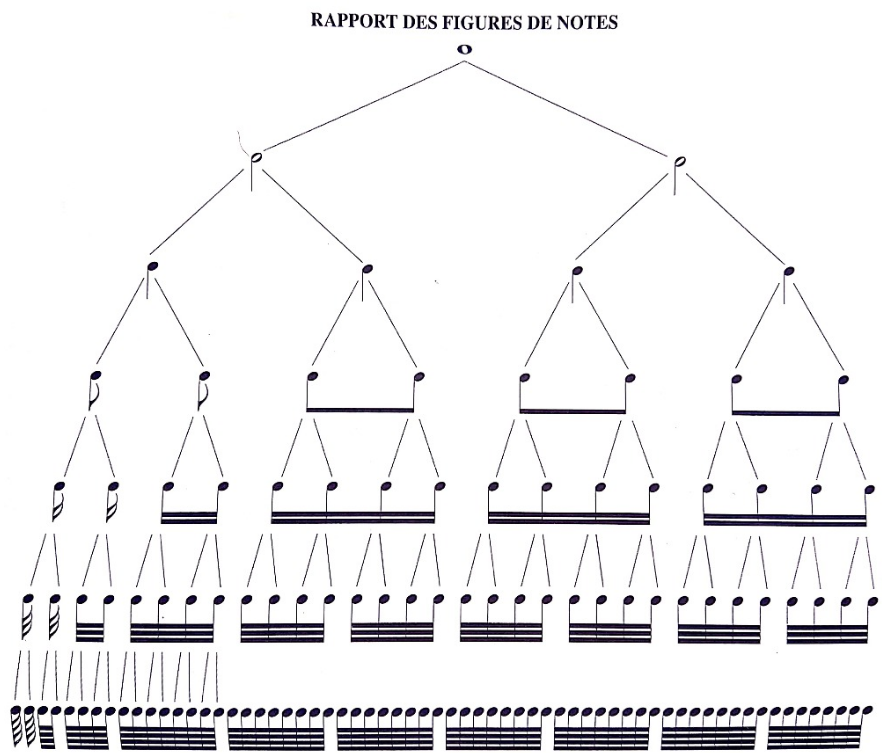
\includegraphics[height=50mm, width=80mm]{
    z_images/3_methodes/0_notation_de_la_batterie/1_rapport_figures_notes.png}
	\caption{Rapport des figures de notes}\cite{danhauser}
	\label{rapp_fig_notes}
\end{figure}

La figure \ref{rapp_fig_notes} montre les rapports de durée entre les figures
de notes. Plus les durées sont longues, plus elles sont marquées par la tête de
note ou la présence ou non de la hampe. À partir de la noire (3ème lignes en
partant du haut), on ajoute un crochet à la hampe d’une figure de notes pour
diviser sa durée par 2. 
Les notes à crochet (croche, double-croche, triple-croche…) 
peuvent être reliées ou non par des ligatures (voir les 4 dernières lignes de
la figure \ref{rapp_fig_notes}).\newpage
\begin{figure}[h]
	\centering
	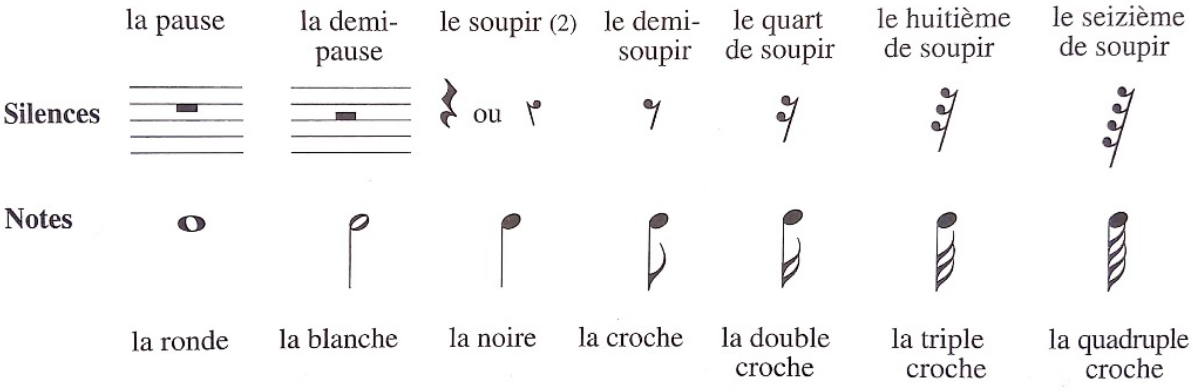
\includegraphics[height=25mm, width=95mm]{
    z_images/3_methodes/0_notation_de_la_batterie/4_silences.png}
	\caption{Les silences}
	\label{silences}
\end{figure}
« Les silences sont des signes qui indiquent l’interruption du son. »
\cite{danhauser}. La figure \ref{silences} montre pour chaque figure de note,
la figure de silence qui lui correspond.\\

La transcription sert à traduire les trois caractéristiques du son musical :
\begin{itemize}
	\item la hauteur, nombre de vibration en un temps donné (son grave ou
        aigu — do, ré, mi,…) ;
	\item l’intensité, amplitude des vibrations (force du son) ;
	\item le timbre, il permet de différencier deux instruments même s’ils
        jouent un son de même hauteur et de même intensité.
\end{itemize}

Ainsi que de leurs combinaisons appelées à former l’ossature de l’œuvre
musicale dans son déroulement temporel, à la fois :
\begin{itemize}
	\item diachronique (succession des instants, ce qui constitue en musique la
        mélodie) ;
	\item et synchronique (simultanéité des sons, c’est-à-dire l’harmonie).
\end{itemize}
\florent{explications sur l’aspect structuré (hiérarchie) : les mesures, les
    groupes ryhtmiques...
         c’est important ici}
\subsubsection*{voix}
Pour les instruments mélodiques, un groupe de notes peut être organisé en
\emph{voix}, représentant des flots mélodiques joués en parallèle, avec une
synchronisation plus ou moins stricte \cite{SHIBATA2021262}
\cite{Guiomard-Kagan}.
\subsubsection*{signature rythmique}
\label{sign_rythm}
<flo>présenter rapidement la notation des signatures rythmiques</flo>
\subsubsection*{appogiatures}
<flo>Parler des appogiatures ici ?</flo>

\subsection*{Les données MIDI}
Le format MIDI\footnote{https://www.midi.org/} est originellement une norme
technique mais peut également être considéré comme une représentation musicale.
Celle-ci peut effectivement être enregistrée par des instruments compatibles,
et visualisée ou jouée par un l’ordinateur. Ce format historique, encore très
largement utilisé, est très important (mais aussi contraignant) dans le cadre
de notre travail, dans la mesure où de nombreux logiciels l'utilisent. Pour la
transcription musicale, il constitue une strate intermédiaire très utile entre
le signal audio (enregistrement) et la représentation musicale lisible par un
humain (partition).

Il s’agit d’un protocole temps réel pour échanger des messages (événement) et
un format de fichier. Un fichier MIDI est une séquence d’évènements datés et il
représente une performance musicale symbolique.

\begin{figure}[h]
	\centering
	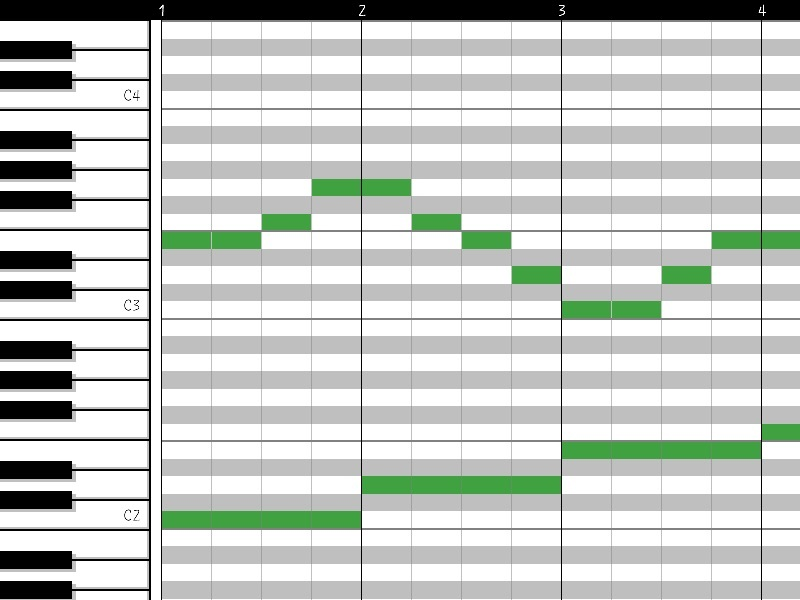
\includegraphics[height=40mm, width=50mm]{
    z_images/1_contexte/2_midi_piano.jpg}
	\caption{Exemple d’évènements MIDI}
	\label{piano_roll}
\end{figure}
Les données midi sont représentées sous forme de piano-roll. Chaque bande verte
sur la figure \ref{piano_roll} correspond à une notes jouée par un instrument.
Le début (onset) et la fin (offset) d’une bande verte sont appelés « évènement
MIDI ». Il existe des évènements ON et des évènements OFF qui ont chacun une
date sur la séquence MIDI. La durée d’une note est représentée la distance
entre les évènements ON et OFF qui lui correspondent.\\

Liste des évènements principaux d’un évènement MIDI :
\begin{itemize}
    \item type de l’évènement, ON ou OFF ;
    \item date de l’évènement, Sa position sur la séquence ;
    \item pitch de l’évènement, à quelle note il correspond (à quelle
        instrument pour la batterie)
    \item velocité, volume sonore de l’évènement.\\
\end{itemize}

\florent{cela pourra être utile d'avoir une
explication (ici ou en 1.4) sur la différence entre les timings de performance
(dont le MIDI non-quantifié est un enregistrement symbolique) et les timing des
partitions. avec 2 unités temporelles différentes (secondes et temps), en
relation par tempo.}

\subsection*{Les formats XML}
<dam>si tu as la date d'apparition du format, éventuellement une citation un
peu originelle</dam>
Il existe plusieurs formats XML dédiés à la musique : MusicXML, MEI, MNX, …

L’inconvénient de ces formats est qu’ils sont verbeux et ambigus, c’est
pourquoi nous utilisons pour la transcription une représentation intermédiaire
abstraite décrite plus loin.


\begin{figure}[h]
	\centering
	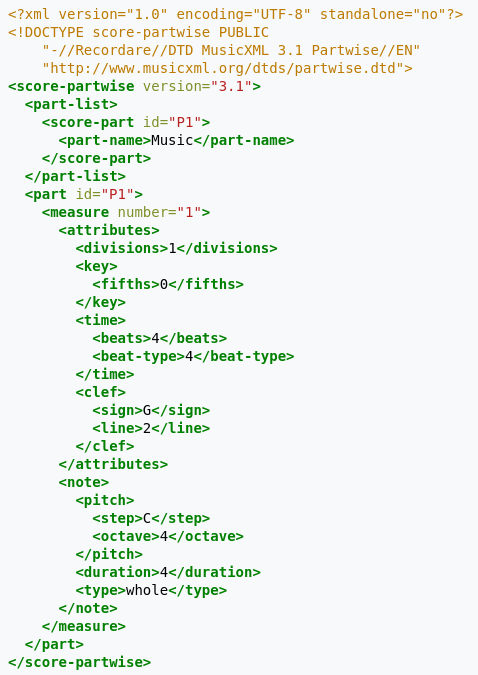
\includegraphics[height=50mm, width=50mm]{
    z_images/1_contexte/6_musicxml_0.png}
    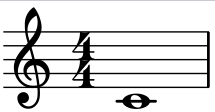
\includegraphics[height=20mm, width=40mm]{
    z_images/1_contexte/6_musicxml_1.png}
	\caption{Exemple de représentation MusicXML} 
	\label{MusicXML}
\end{figure}

Le figure \ref{MusicXML}
\footnote{\textit{Source images :
\url{https://fr.wikipedia.org/wiki/MusicXML}}}
représente un do en clef de sol de la durée d’une ronde sur une mesure en 4/4
écrit au format MusicXML.
Un des avantages de ce format est qu’il peut être converti aussi bien en
données MIDI qu’en partition musicale, ce qui en fait un bon format
intermédiaire pour manipuler les données musicales et les échanger entre les
programmes.
<dam>c'est un peu ce que je mettais plus haut pour le MIDI, là on a une autre
représentation, moins "audio" et plus "musique" bref tu peux développer cet
aspect de représentation formelle et le questionner un peu.
si tu as le temps et l'envie, tu pourrais poser le problème. qu'est)ce qu'une
bonne représentation (et informatisable) de la musiqu ? quels sont les
avantages / inconvénients de MIDI / MusicXML ?
et enfin, la question centrale que tu pourrais déjà évoquer ici : dans quelle
mesure les correspondances MIDI <=> MusicXML sont elles univoques, ou y-a-t-il
plusieurs choix possibles (spoiler oui)</dam>

\section*{Conclusion}
Dans ce chapitre, nous avons établi que la RIM a connu un fort développement
ces dernières années, et qu'il s'inspire de plus en plus de méthodes TAL, et
que, par ce biais, il y a des liens possibles entre le traitement du langage
musical et celui des langues naturelles, le plus proche étant probablement le
phénomène de transcription (par analogie avec le \textit{speech to text}).


\chapter{État de l’art}
\label{etat_de_l_art}
\minitoc
\section*{Introduction}
Dans ce chapitre, nous présenterons quelques travaux antérieurs dans le domaine
de la transcription automatique de la musique et de la batterie afin de situer
notre démarche.

Nous aborderons le passage crucial du monophonique au polyphonique dans la
transcription. Nous ferons un point sur les deux grandes parties de la TAM de
bout en bout : de l’audio vers le MIDI puis des données MIDI vers l’écriture
d’une partition. Ensuite, nous discuterons des approches linéaires et des
approches hiérarchiques.

\section{Monophonique et polyphonique}
Les premiers travaux en transcription ont été faits sur l’identification des
instruments monophoniques\footnote{Instruments produisant une note à la fois,
ou plusieurs notes de même durée en cas de monophonie par accord (flûte,
clarinette, sax, hautbois, basson, trombone, trompette, cor, etc…)}
\cite{future_directions}. Actuellement, le problème de l'estimation automatique
de la hauteur des signaux monophoniques peut être considéré comme résolu, mais
dans la plupart des contextes musicaux, les instruments sont polyphoniques
\footnote{guitare, piano, basse, violon, alto, violoncelle, contrebasse,
glockenspiel, marimba, etc…}. L'estimation des hauteurs multiples est le
problème central de la création d'un système de transcription de musique
polyphonique. Tout signal audio musical peut être composé de plusieurs signaux,
ceux-ci pouvant provenir de plusieurs instruments, ou d'un instrument dit
polyphonique. Une tâche difficile consiste à séparer, à partir du signal, les
différentes sources (ou voix) afin de les représenter individuellement. La
batterie, composée de plusieurs instruments (caisse claire, grosse caisse,
cymbales, toms, etc…), est un cas typique d'intrument polyphonique pour lequel
ce défi est majeur .

Les performances des systèmes actuels ne sont pas encore suffisantes pour
permettre la création d'un système automatisé capable de transcrire de la
musique polyphonique sans restrictions sur le degré de polyphonie ou le type
d'instrument. Cette question reste donc encore ouverte.

\section{De l’enregistrement audio vers le MIDI}
\label{audio_to_midi}
Jusqu’à aujourd’hui, les recherches se sont majoritairement concentrées sur le
traitement de signaux audio vers la génération de contenu MIDI non-quantifié
(une performance — à expliquer) \cite{AMT_for_2_Instru}. Cette tâche englobe
plusieurs sous-tâches dont séparation des sources audio, la détection
multi-\textit{pitchs} \footnote{La détection multi-\textit{pitchs} est la
détection des hauteurs simultanées pour les instruments polyphoniques. Il peut
s’agir de notes d’un même instrument ou de plusieurs instruments différents.}
et la détection des \textit{onsets} et des \textit{offsets}.

\florent{avant la TAB, il faudrait dire 2 mots sur les techniques utilisées
(cf. survey AMT Benetos et al.)}

En transcription automatique de la batterie \cite{Review_ADT}, plusieurs
stratégies de répartition pré/post-\textit{processing} sont possibles pour la
détection multi-\textit{pitchs}. La détection peut être entamée dès le
pré-\textit{processing}, en supprimant les \textit{features}\footnote{
Features : caractéristiques individuelles mesurables d'un phénomène dans le
domaine de l'apprentissage automatique et de la reconnaissance des formes}
non-pertinentes pendant la séparation des sources afin d’obtenir une meilleure
détection des instruments de la batterie, par exemple en supprimant la
structure harmonique pour atténuer l’influence des instruments à hauteurs sur
la détection grosse caisse et caisse claire. Mais certaines études montrent que
la suppression des instruments à hauteurs peut avoir des effets néfastes sur
les performances de la transcription de batterie. En outre, les systèmes de TAB
basés sur des réseaux de neurones récurrents ou sur des factorisations
matricielles font la séparation des sources pendant l’optimisation, ce qui
réduit la nécessité de la faire pendant le pré-processing. Pour la
reconnaissance des instruments de la batterie, une autre approche possible est
d’utiliser un modèle probabiliste (MMC) pour classifier les différents sons de
la batterie \cite{Eronen}. L’approche AdaMa \cite{adama_1}, qui commence par
une estimation initiale des sons de la batterie en les raffinant itérativement,
est une autre approche de la même catégorie.

Toutes ces méthodes elles visent toutes la génération d’un contenu MIDI
non-quantifié qui est la représentation symbolique d’une performance musicale.

\section{Du format MIDI vers une partition}
Les approches mentionnées en section \ref{audio_to_midi} produisent en sortie
un fichier MIDI non-quantifié, qui est un format encore très éloigné d'une
partition musicale. Un premier problème concerne les timings (dates et durées
d'événements) qui doivent être alignées à des positions temporelles
correspondant à des valeurs exprimables avec la notation musicale (voir la
différence entre contenu MIDI et musique écrite en section 1.4). On parle de
quantification rhythmique.

Nakamura et al. 2016 présentent une approche de quantification rhythmique avec
modèles de probabilités (MMC) qui prend en entrée un fichier MIDI non quantifié
et fourni en sortie un fichier MIDI quantifié. \cite{SHIBATA2021262} étendent
ensuite l'approche à une transcription d'enregistrement audio vers un fichier
MIDI quantifié. Ce dernier format, linéaire, ne correspond toutefois pas encore
à une partition structurée,  avec groupement rythmiques hérarchiques (voir la
section 1.4). Dans ces travaux, la structuration des données en partition est
déléguée à un éditeur de partitions (MuseScore), avec des résultats assez
inégaux.

Seuls quelques travaux récents s’intéressent de près à la création d’outils
permettant la génération de partition. Le problème de la conversion d'une
séquence d'évènements musicaux symboliques en une partition musicale structurée
est traité notamment dans \cite{foscarin:hal-01988990}. Ce travail, qui vise à
résoudre de manière conjointe la quantification rythmique et la production de
partitions structurées, s’appuie tout au long du processus sur des grammaires
génératives qui fournissent un modèle hiérarchique — langage a priori des
partitions. Les expériences ont des résultats prometteurs, mais il faut relever
qu’elle ont été menées avec un ensemble de données composé d'extraits
monophoniques ; Il reste donc à traiter le passage au polyphonique, qui
nécessite de traiter le problème supplémentaire de la séparation de voix,
\florent{i.e. pour la batterie on nveut quantification + structuration +
    séparation mais seules les 2 premières sont couplées dans l'approche de
    ton stage.}
en le couplant avec la quantification du rythme.

L'approche de \cite{foscarin:hal-01988990} est fondée sur la conviction 
que la complexité de la structure musicale dépasse les modèles linéaires.

\section{Approche linéaire et approche hiérarchique}

\begin{figure}[h]
	\centering
	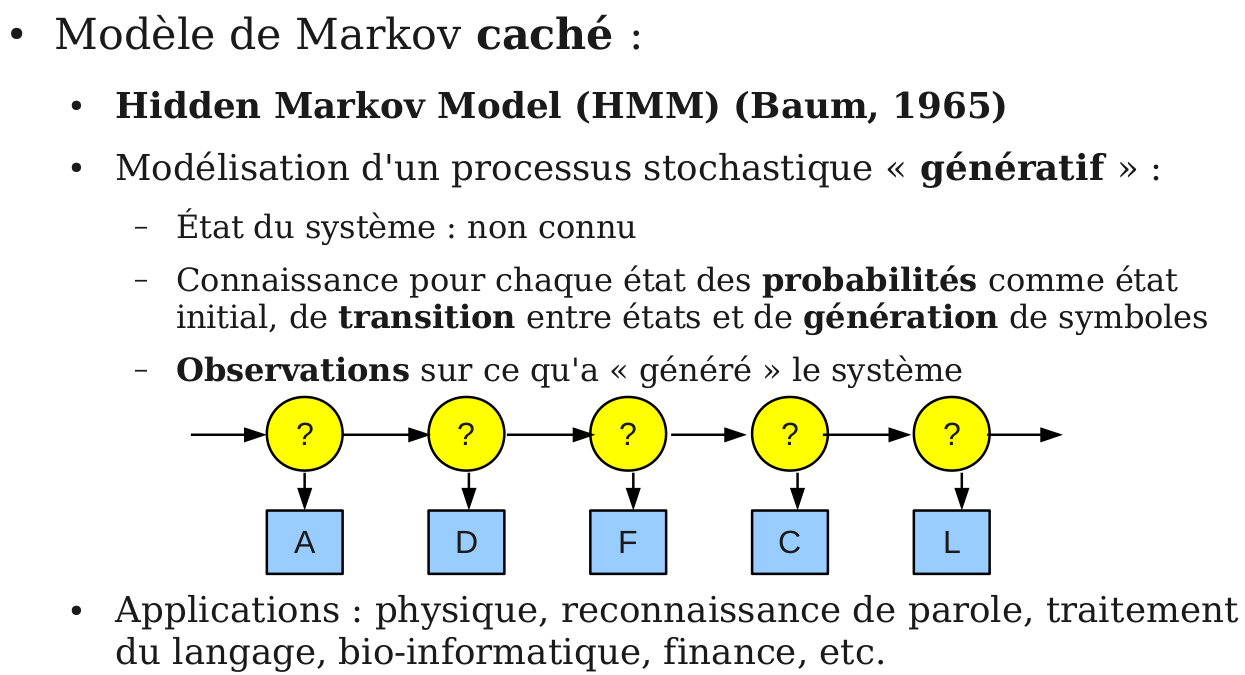
\includegraphics[height=50mm, width=90mm]{
    z_images/2_etat_de_l_art/0_hmm.png}
	\caption[Le modèle de Markov caché]{Le modèle de Markov caché\footnotemark}
    \label{mmc}
\end{figure}

<dam>qu'est-ce q'un modèle linéaire</dam>\\
La figure \ref{mmc} montre un exemple de modèle linéaire et mentionne notamment
ce type de modèle sont utilisé en reconnaissance de la parole. Une différence
notable entre la reconnaissance de la parole et le traitement de la musique est
que la parole est un type de données linéaires : les informations sonores
arrivent les unes après les autres. Mais l’expression musicale provient en
grande partie du mélange des sons. Certaines information musicales sont
nécessairement issues de plusieurs sons produit simultanément.

Plusieurs travaux ont d’abord privilégié l’approche stochastique. Par exemple,
Shibata \textit{et al.} \cite{SHIBATA2021262} ont utilisé des MMC pour la
reconnaissance des signatures rythmiques. Les auteurs utilisent d’abord deux
réseaux de neurones profonds, l’un pour la reconnaissance des \textit{pitchs}
et l’autre pour la reconnaissance de la vélocité. Ils construisent ensuite
plusieurs MMC étendus pour la musique polyphonique correspondant à des
signatures rythmiques possibles, puis ils calculent la probalitité maximale
pour chaque modèle afin d’obtenir la signature rythmique la plus probable.\\

L’évaluation finale des résultats de \cite{SHIBATA2021262} montre qu’il faut
\footnotetext{Source : cours de Damien Nouvel
\url{https://damien.nouvels.net/fr/enseignement}}
rediriger l’attention vers les valeurs des notes, la séparation des voix et
d'autres éléments délicats de la partition musicale qui sont significatifs pour
son interprétation.

Même si la quantification du rythme se fait le plus souvent par la
manipulation de données linéaires, de nombreux travaux suggèrent d’utiliser
une approche hiérarchique puisque le langage musical est lui-même structuré.

\florent{je ne comprend pas bien l'explication. le pb est plutot vue locale 
(déduction de la proba d'une durée à partir de la durée précédente, par ex.
dans un MMC) 
vs vue globale, dans une hiérarchie}

En effet, l’usage d’arbres syntaxiques semble approprié pour représenter le
langage musical. Une méthodologie simple pour la description et l'affichage des
structures musicales est présentée dans \cite{rythm_tree}. 
Les arbres de rythmes y sont évoqués comme permettant une cohésion complète de
la notation musicale traditionnelle avec des notations plus complexes.
Jacquemard \textit{et al.} \cite{jacquemard:hal-01134096} propose aussi une
représentation formelle du rythme, inspirée de modèles théoriques antérieurs
issus du domaine de la réécriture de termes. 
\florent{techniques de réécriture: appliquée à la déduction automatique, calcul
symbolique} Ils montrent aussi qu'il est possible d'appliquer des arbres de
rythmes pour le calcul d'équivalences rythmiques dans
\cite{jacquemard:hal-01403982}. La réécriture d’arbres, dans un contexte de
composition assistée par ordinateur, par exemple, pourrait permettre de
suggérer à un utilisateur diverses notations possibles pour une valeur
rythmique, avec des complexités différentes.

La nécessité d’une approche hiérarchique pour la production automatique de
partition est évoquée dans \cite{foscarin:hal-01988990}. 
\florent{citer thèse de David Rizo (Valencia)}
Les modèles de grammaire qui y sont exposés sont différents de modèles
markoviens linéaires de précédents travaux.
\begin{figure}[h]
	\centering
	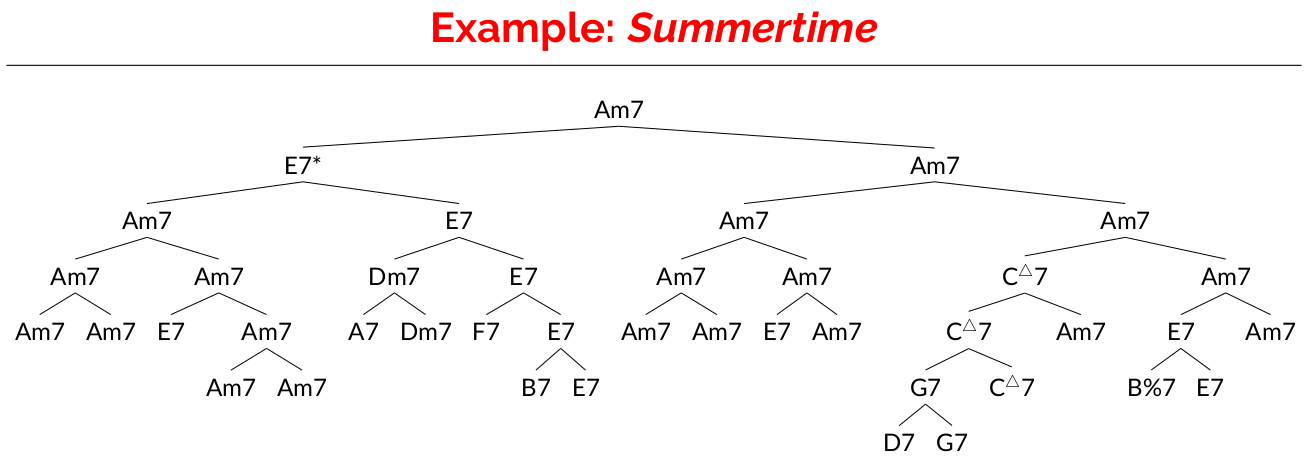
\includegraphics[height=40mm, width=120mm]{
    z_images/2_etat_de_l_art/1_summertime_tree.png}
	\caption{arbre\_jazz}
	\textit{Représentation arborescente d’une grille harmonique}
    \cite{harasimjazz}
\end{figure}
<dam>il serait mieux de citer cette figure et de la commenter un peu</dam>

\section*{Conclusion}
La plupart des travaux déjà existants sur la TAB ont été énumérés par Wu
\textit{et al.} \cite{Review_ADT} qui, pour mieux comprendre la pratique des
systèmes de TAB, se concentrent sur les méthodes basées sur la factorisation
matricielle et celles utilisant des réseaux neuronaux récurrents. La majorité
de ces recherches se concentre sur des méthodes de calcul pour la détection
d'événements sonores de batterie à partir de signaux acoustiques ou sur la
séparation entre les évènements sonores de batterie avec ceux des autres
instruments dans un orchestre ou un groupe de musique \cite{2802}, ainsi que
sur l'extraction de caractéristiques de bas niveau telles que la classe
d'instrument et le moment de l'apparition du son. Très peu d'entre eux ont
abordé la tâche de générer des partitions de batterie et, même quand le sujet
est abordé, l’output final n’est souvent qu’un fichier MIDI non-quantifié et
non une partition écrite.

%\florent{diff. pour production de partition (et 1 des obj. du stage) est...}
En conclusion, il n’existe pas de formalisation de la notation de la batterie
ni de réelle génération de partition finale, dont les enjeux principaux
seraient :
\begin{enumerate}
    \item le passage du monophonique au polyphonique, comprenant la distinction
        entre les sons simultanés et les appogiatures ou autres ornements ;
    \item les choix d’écritures spécifiques à la batterie concernant la
        séparation des voix et les continuations.
\end{enumerate}


\chapter{Méthodes}
\label{methodes}
\minitoc
\section*{Introduction}
Dans ce chapitre, nous expliquerons en détail les méthodes que nous avons
employées pour l’ADT.\\
Pour commencer, nous exposerons une description de la notation de la batterie
ainsi qu’une modélisation de celle-ci pour la représentation des données
rythmiques en arbres syntaxiques. Nous poursuivrons avec une présentation de
qparse\footnote{https://qparse.gitlabpages.inria.fr/}, un outil de
transcription qui est développé à l'Inria, l'Université de Nagoya et plusieurs
développeurs au sein du laboratoire Cedric au CNAM.

Enfin, nous présenterons les \textbf{formes rythmiques}, <flo>une
représentation
théorique qui permet…</flo> 

\section{La notation de la batterie}
\label{notation_batterie}
Pour la transcription, j’ai choisi d’utiliser une notation inspirée du recueil
de pièces pour batterie de J.-F. Juskowiak \cite{jusko} et des méthodes de
batterie Agostini \cite{ago_meth_3}, car je trouve la position des éléments
cohérente et intuitive (voir section \ref{hauteurs}).\newpage

%\subsection*{Les hauteurs et les têtes de notes}
%\label{hauteurs}
\begin{figure}[h]
\centering
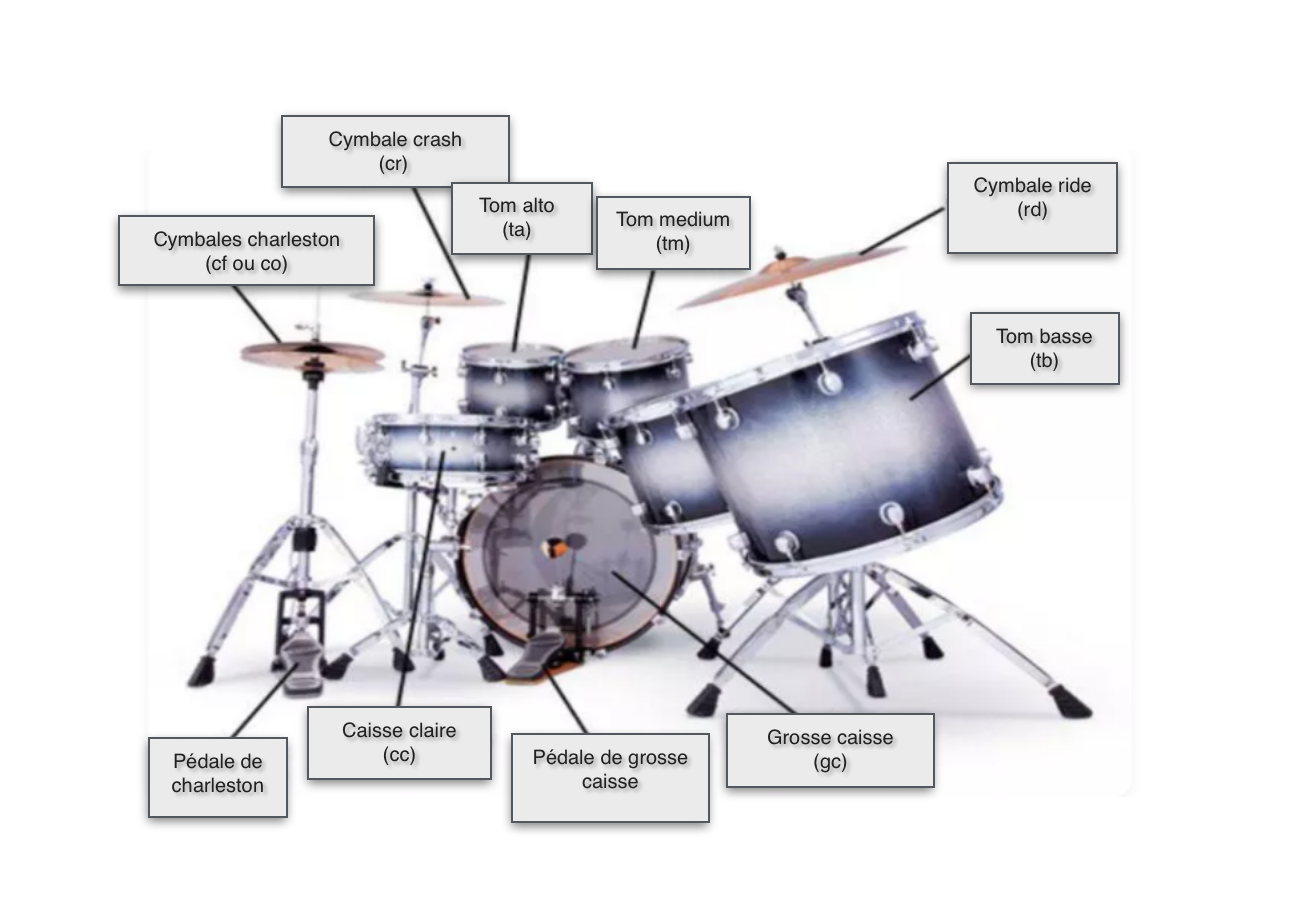
\includegraphics[height=69mm, width=115mm]{
z_images/3_methodes/0_notation_de_la_batterie/batterie.png}
\caption{Les instruments de la batterie}
\label{instru_batt}
\end{figure}

\begin{figure}[!h]
\centering
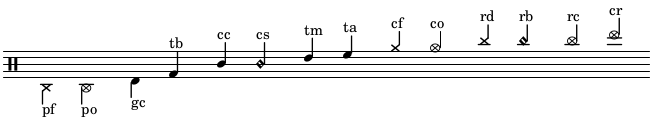
\includegraphics[height=25mm, width=130mm]{
z_images/3_methodes/0_notation_de_la_batterie/2_hauteurs_et_tete_de_notes.png}
\caption{Hauteur et têtes de notes}
\label{haut}
\end{figure}

\begin{table}[h]
\centering
\begin{tabular}{|c|c|c|} \hline
Noms figure \ref{instru_batt} & codes figure \ref{haut}  & référence \\ \hline
Pédale de charleston & pf ou po & charley fermé ou ouvert au pied \\
Grosse caisse & gc & grosse caisse \\
Tom basse & tb & tom basse \\
Caisse claire & cc & caisse claire \\
Tom médium & tm & tom médium \\
Tom alto & ta & tom alto \\
Cymbales charleston & cf ou co & charley fermé ou ouvert à la main \\
Cymbales ride & rd & ride \\
Cymbales crash & cr & crash \\ \hline
	\end{tabular}
	\caption{Noms des instruments de la batterie}
	\label{nom_instru_batt}
\end{table}\newpage
La figure \ref{instru_batt}\footnote{Source : \url{
https://www.superprof.fr/blog/composition-instrument-percussion/}} montre une
batterie standard avec tous les instruments habituellement présent sur une
batterie et la figure \ref{haut} donne leur représentation sur une partition.

Le tableau \ref{nom_instru_batt} donne dans l’ordre :
\begin{enumerate}
    \item les noms des instruments sur la figure \ref{instru_batt} ;
    \item leurs codes respectifs dans la figure \ref{haut} ;
    \item les noms que j’utiliserai dans le présent document pour y référer.
\end{enumerate}
Les figures \ref{instru_batt}, \ref{haut} et le tableau \ref{nom_instru_batt}
peuvent aider à comprendre pourquoi je trouve la notation agostinienne
cohérente et intuitive.

En effet, les hauteurs sur la portée représentent :
\begin{enumerate}
	\item La hauteur physique des instruments :\\
	La caisse claire est centrale sur la portée et sur la batterie (au niveau
    de la ceinture, elle conditionne l’écart entre les pédales et aussi la
    position de tous les instruments basiques d’une batterie).\\
	Tout ce qui en-dessous de la caisse claire sur la portée est en dessous de
    la caisse claire sur la batterie (pédales, tom basse) ;\\
	Tout ce qui est au-dessus de la caisse claire sur la portée, l’est aussi
    sur la batterie.\\
	\item La hauteur des instruments en terme de fréquences :\\
	Sauf pour le charley au pied et si l’on sépare en trois groupes
    (grosse caisse, toms et cymbales), de bas en haut, les instruments vont du
    plus grave au plus aigu.
\end{enumerate}

\subsection*{Les durées}
\label{hho}
Comme nous venons de la voir, la majorité des instruments de la batterie sont
représentés par les têtes des notes. De plus, le seul instrument dont le son
peut être arrêté de manière quantifiée et dont la durée sonore nous intéresse
est le charley\footnote{Je ne prendrais pas en compte l’arrêt des cymbales à la
main car ce phénomène n’existe pas dans les fichiers MIDI.}.
\florent{certaines têtes de notes vides alors que leur durée n'est pas celle
des blanches? expliquer les différences avec la notation conventionnelle cf
1.4}

Par conséquent :
\begin{enumerate}
    \item les durées — sauf pour le charley — représenterons un écart temporel
        entre les notes et non une durée sonore et elles pourront donc être
        rallongée à l’aide de silences ;
    \item les symboles rythmiques concernant les têtes de note ne pourront pas
        être utilisés pour exprimer les durées. Cela est valable aussi pour la
        présence ou non de la hampe puisque ce phénomène n’existe qu’avec les
        têtes de notes de type cercle-vide (opposition blanche-ronde). L’usage
        des blanches existe dans certaines partitions de batterie
        \cite{system_drums} mais cela reste dans des cas très rares. Certains
        logiciels permettent de faire des blanches avec des symboles
        spécifiques à la batterie ou aux percussions mais leur lecture reste
        peu aisée et leur utilisation pour la batterie est rarissime.\\
\end{enumerate}

En résumé :
\begin{itemize}
    \item toutes les notes ont une hampe ;
    \item une notes dont la hampe n’a pas de crochet est toujours une noire ;
    \item à part pour le charley ouvert, les durées n’expriment pas la durée
        d’un son mais une distance temporelle entre deux notes.
    \item à part pour le charley ouvert, la durée d’une note peut être
        prolongée par un silence (exemple : une noire + un soupir pour exprimer
        une blanche)\\
\end{itemize}
La durée d’une note peut être prolongée par divers symboles :
\begin{itemize}
	\item Le point : il rallonge la durée d’une note de la moitié de sa valeur.
        Dans la deuxième note de l’exemple 3 de la figure \ref{point_liaison}
        est une noire pointée, elle vaut donc la durée d’une noire + une croche
        (ou de trois croche) ;
	\item La liaison : elle rallonge la durée de la première note de la durée
        de la deuxième. La deuxième note de l’exemple 4 de la figure
        \ref{point_liaison} est une croche qui est liée à une noire, sa durée
        est donc équivalente à celle d’une croche + une noire (ou de trois
        croches) ;
    \item les silences (pas pour les ouvertures de charley).
\end{itemize}

\begin{figure}[h]
	\centering
	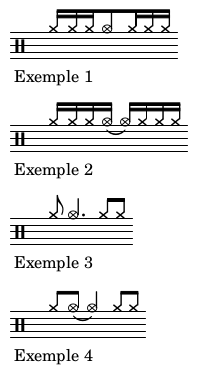
\includegraphics[height=80mm, width=40mm]{
    z_images/3_methodes/0_notation_de_la_batterie/3_point_et_liaison.png}
	\caption{Point et liaison}
	\label{point_liaison}
\end{figure}

Un autre élément concernant la notation des durées en batterie est la nécessité
de faire ressortir la pulsation\footnote{La position des temps} de la rendre
visuelle. La première chose à prendre en compte pour analyser la figure
\ref{point_liaison} est donc la nécessité de regrouper les notes par temps à
l’aide des ligatures. Le deuxième point est de s’arranger pour qu’il y ait une
indication visuelle au début de chaque temps.

\begin{itemize}
    \item Exemple 1 : l’ouverture de charley est quantifiée mais les notes ne
        sont pas regroupées par temps.
    \item Exemple 2 : Ici, la liaison permet de regrouper les notes par temps
        en obtenant le même rythme que dans l’exemple 1.
    \item Exemple 3 et exemple 4 : les deux exemples sont valables mais le
        deuxième est le plus souvent utilisé car la liaison donne un repair
        visuel sur le temps.\\
\end{itemize}

En cas de nécessité de prolonger la durée d’une note au-delà 
de son temps de départ (syncope) et si cette note ne correspond pas à une
ouverture de charley, elle sera prolongerée sur le temps suivant à l’aide de
silences dont le premier sera positionné sur le temps. Si la note syncopée est
une ouverture de charley, on privilégiera la liaison pour sa prolongation.

\subsection*{Les silences}
Les silences sont parfois utilisés pour noter les fermetures de charley (après
une ouverture). Les fermetures du charley sont notées soit par un silence
(correspondant à une fermeture de la pédale), soit par un écrasement de
l’ouverture par un autre coup de charley fermé, au pied ou à la main.

\begin{figure}[h]
	\centering
	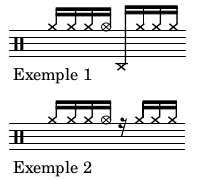
\includegraphics[height=40mm, width=40mm]{
    z_images/3_methodes/0_notation_de_la_batterie/5_silence_joue.png}
	\caption{Silence joué}
	\label{silence joue}
\end{figure}

L’écriture littérale de contenu MIDI peut ressembler à l’exemple 1 de la figure
\ref{silence joue}. Sur cet exemple, le son de l’ouverture de charley est
arrêté par une pression du pied sur la pédale et c’est ce que le batteur joue
dans les faits. Mais il apparaît intuitivement que le but de la première note
du deuxième temps n’est pas de générer un son de charley au pied mais
uniquement de stopper l’ouverture. La notation de l’exemple 2 de la figure
\ref{silence joue} serait donc préférable car elle représente mieux l’intention
de ce rythme et elle n’empiète pas sur une potentielle voix basse qui pourrait
le compléter (on évite une écriture surchargée).

Lorsqu’une note est un charley ouvert, il faudra donc prendre en compte la note
suivante pour l’écriture :
\begin{enumerate}
    \item si c’est un charley fermé joué à la main $\Rightarrow$ la note sera
        un charley fermé joué à la main (cf) ;
    \item si c’est un charley fermé joué au pied $\Rightarrow$ la note sera un
        silence.
\end{enumerate}
La deuxième règle sera soumise au cadre imposé par certaines
\textbf{formes rythmiques} pour lesquelles le charley joué au pied devra rester
tel quel. 

\subsection*{Les équivalences rythmiques}
Pour les instruments mélodiques, dans le cas de notes dont la durée de l’une à
l’autre est ininterrompue et si leur durée initiale est prolongée, seuls la
liaison et le point permettent des notations équivalente. Mais pour la
batterie et à part dans le cas des ouvertures de charley (voir section
\ref{hho}), seules comptent des dates de début (onsets) : la durée du son n’a
pas d’importance. L’usage des silences pour combler la distance rythmique entre
deux notes devient donc possible.

Cela pris en compte, et étant donné que les indications de durée dans les têtes
de notes sont peu recommandées (voir section \ref{hho}), l’écriture à l’aide de
silences sera privilégiée comme indication de durée sauf dans les cas où cela
reste impossible. Ce choix à pour but de n’avoir qu’une manière d’écrire toutes
les notes, quelles que soient leur tête de note (sauf pour le charley).

\begin{figure}[h]
	\centering
	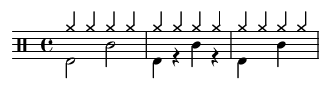
\includegraphics[height=20mm, width=75mm]{
    z_images/3_methodes/0_notation_de_la_batterie/6_equivalence.png}
	\caption{Équivalence}
	\label{equivalence}
\end{figure}

Sur la figure \ref{equivalence}, théoriquement, il faudra choisir la notation
de la deuxième mesure mais dans certains contextes, pour des raisons de
lisibilité ou de surcharge, la version sans les silences de la troisième mesure
pourra être choisie.

\subsection*{Les voix}
Pour les instruments mélodiques, un groupe de notes peut être organisé en
\emph{voix}, représentant des flots mélodiques joués en parallèle, avec une
synchronisation plus ou moins stricte \cite{SHIBATA2021262}
\cite{Guiomard-Kagan}.
% voir ref [15] ou [16] de SHIBATA….

En batterie, une voix est théoriquement l’ensemble des instruments qui, à eux
seuls, constituent une phrase rythmique. Mais en pratique, les instruments
peuvent aussi être divisés par voix dans le but de ne pas surcharger la
notation ou pour que leur disposition soit représentée sur la
partition (voir section \ref{notation_batterie}).
Les voix sont charactérisées par l’orientation des hampes et plus présicément
par les ligatures si les hampes sont dans la même direction (voir figure
\ref{afro_latin}).

\begin{figure}[h]
	\centering
	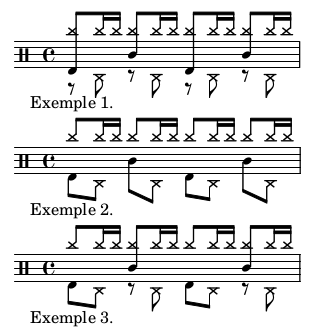
\includegraphics[height=65mm, width=60mm]{
    z_images/3_methodes/0_notation_de_la_batterie/7_voix.png}
	\caption{Séparation des voix}
	\label{sep_voix}
\end{figure}
Sur la figure \ref{sep_voix}, il faudra faire un choix entre les exemples 1, 2
et 3 qui sont trois façons équivalentes d’écrire le même rythme.
Ce choix se fera en fonction des instruments joués, de la nature plus ou moins
systèmatique de leurs phrasés, et des associations logiques entre les
instruments dans la distribution des rythmes sur la batterie (voir la section
\ref{sys_sep_voix}).

\subsection*{Les accentuations et les ghost-notes}
« Certaines notes dans une phrase musicale doivent, ainsi que les différentes
syllabes d’un mot, être accentuées avec plus ou moins de force, porter une
inflexion particulière. » \cite{danhauser}
\begin{figure}[h]
\centering
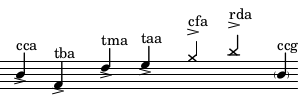
\includegraphics[height=25mm, width=75mm]{
z_images/3_methodes/0_notation_de_la_batterie/8_accents_et_ghost-notes_0.png}
\caption{Les accents et les ghost-notes}
\label{accents_et_gn}
\end{figure}

Théoriquement, tous les instruments peuvent être accentués (voir la section
\ref{velocite}), mais la figure \ref{accents_et_gn} représentent ceux dont les
accents ne demandent pas un grand niveau de maîtrise et sont presque toujours
bien articulés. En outre, les instruments qui ne sont pas représentés sur cette
figure ne sont presque jamais accentués dans les partitions et ne sont pas
présents de manière significative dans le GMD.

Les accents sont marqués par le symbole~«~>~». Ils sont positionnés au-dessus
des notes représentant des cymbales et en-dessous des notes représentant des
toms ou la caisse claire. Ce choix a été fait pour la partition de la figure
\ref{partition_ref} car elle est plus lisible ainsi, mais ces choix devront
être adaptés en fonction des différentes \textbf{formes rythmiques} reconnues
(voir la section \ref{systemes_methodes}). Par exemple, pour les
\textbf{formes rythmiques} jazz, les ligatures pour les toms et la caisse
claire seront dirigées vers le bas, il faudra donc mettre les symboles
d’accentuation correspondants au-dessus des têtes de notes.

La dernière note de la figure \ref{accents_et_gn} montre un exemple de notation
pour une ghost note jouée à la caisse claire. Une ghost note
\cite{lexique_drum} est une note de faible volume sonore mais jouée fermement.
Les ghost notes servent le plus souvent à donner le débit d’un rythme (ses
subdivisions) pour le rendre plus dansant (lui donner plus de « groove » ou de
« swing »). Le parenthésage a été choisi car il peut être utilisé sur n’importe
quelle note sans changer la tête de note.

Toutes les notes de la figure \ref{accents_et_gn} sont exposées en situation
réelle dans la figure \ref{exemple_acc_et_gn}. 
\begin{figure}[h]
\centering
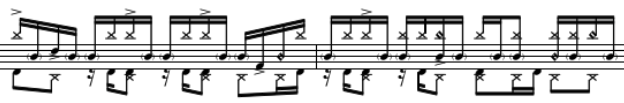
\includegraphics[height=20mm, width=110mm]{
z_images/3_methodes/0_notation_de_la_batterie/8_accents_et_ghost-notes_1.png}
\caption{Exemple pour les accentuations et les ghost-notes}
\label{exemple_acc_et_gn}
\end{figure}

\subsection*{Les flas}
Le fla est appogiature qui consiste à jouer deux coups presque simultanés dont
le premier est une ghost note et le deuxième une note normale ou accentuée.
\begin{figure}[h]
    \centering
    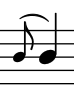
\includegraphics[height=10mm, width=8mm]{
    z_images/3_methodes/0_notation_de_la_batterie/fla_def.png}
    \caption{Définition du fla}
\end{figure}

\section{La transcription manuelle}
Mis à part les figures du chapitre 1 et certains exemples d’analyses de la
section \ref{analyses_et_TM}, toutes les partitions et figures de ce document
ont généré avec lilypond\footnote{\url{http://lilypond.org/index.fr.html}}.\\

\subsection*{Présentation de lilypond}
« LilyPond est un logiciel de gravure musicale, destiné à produire des
partitions de qualité optimale. Ce projet apporte à l’édition musicale
informatisée l’esthétique typographique de la gravure traditionnelle. LilyPond
est un logiciel libre rattaché au projet GNU. »\\

En raison de :
\begin{itemize}
    \item notation agostini
    \item grande liberté de choix
    \item …
\end{itemize}

Lilypond est actuellement le meilleur de logiciel de gravure musicale pour la
batterie.

\begin{figure}[h]
    \centering
    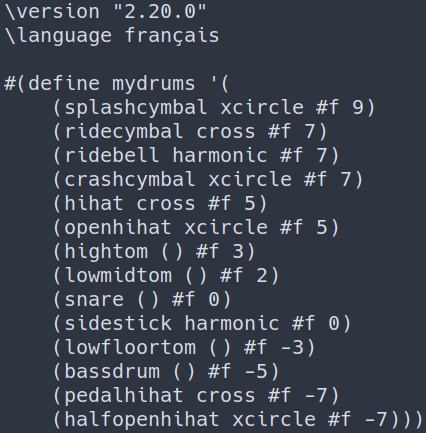
\includegraphics[height=40mm, width=30mm]{
    z_images/3_methodes/transcription_manuelle/drum_perso_1}
    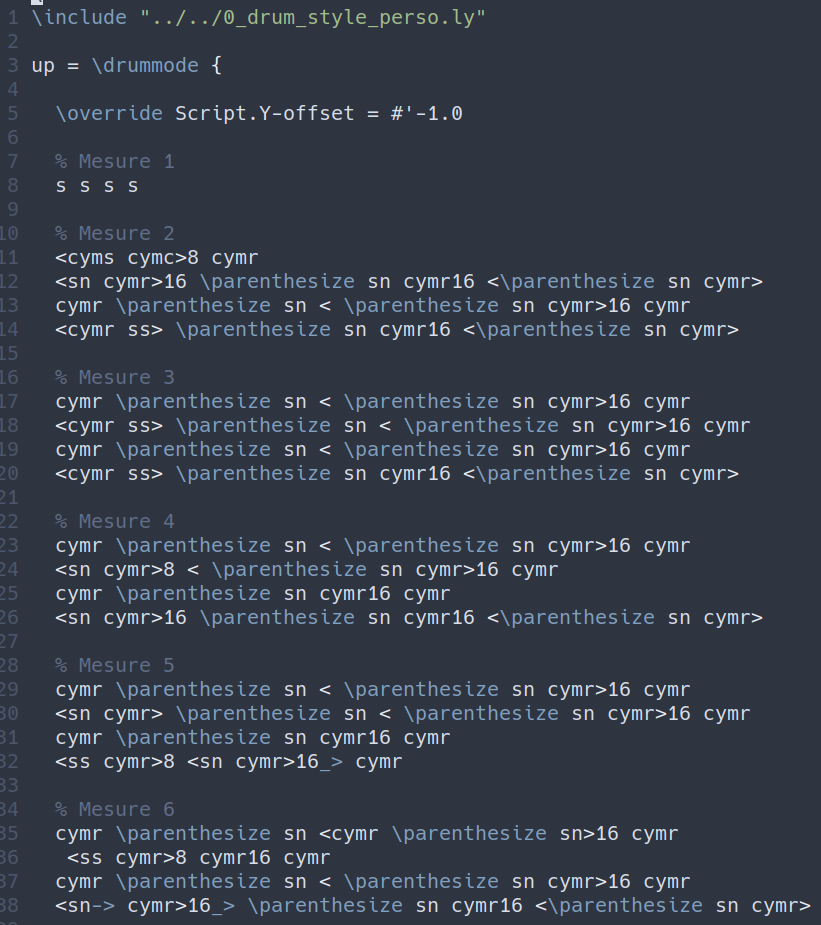
\includegraphics[height=70mm, width=50mm]{
    z_images/3_methodes/transcription_manuelle/extrait_code.png}
    \caption{lilypond — extraits de code}
    \label{extrait_code}
\end{figure}

Sur la figure \ref{extrait_code} :
\begin{itemize}
    \item à gauche : configuration aménagée pour la notation de type agostini.
    \item à droite : le début de code mesure par mesure pour la voix haute
        d’une partition (en haut du fichier, inclusion du fichier de config)
\end{itemize}

\begin{figure}[h]
    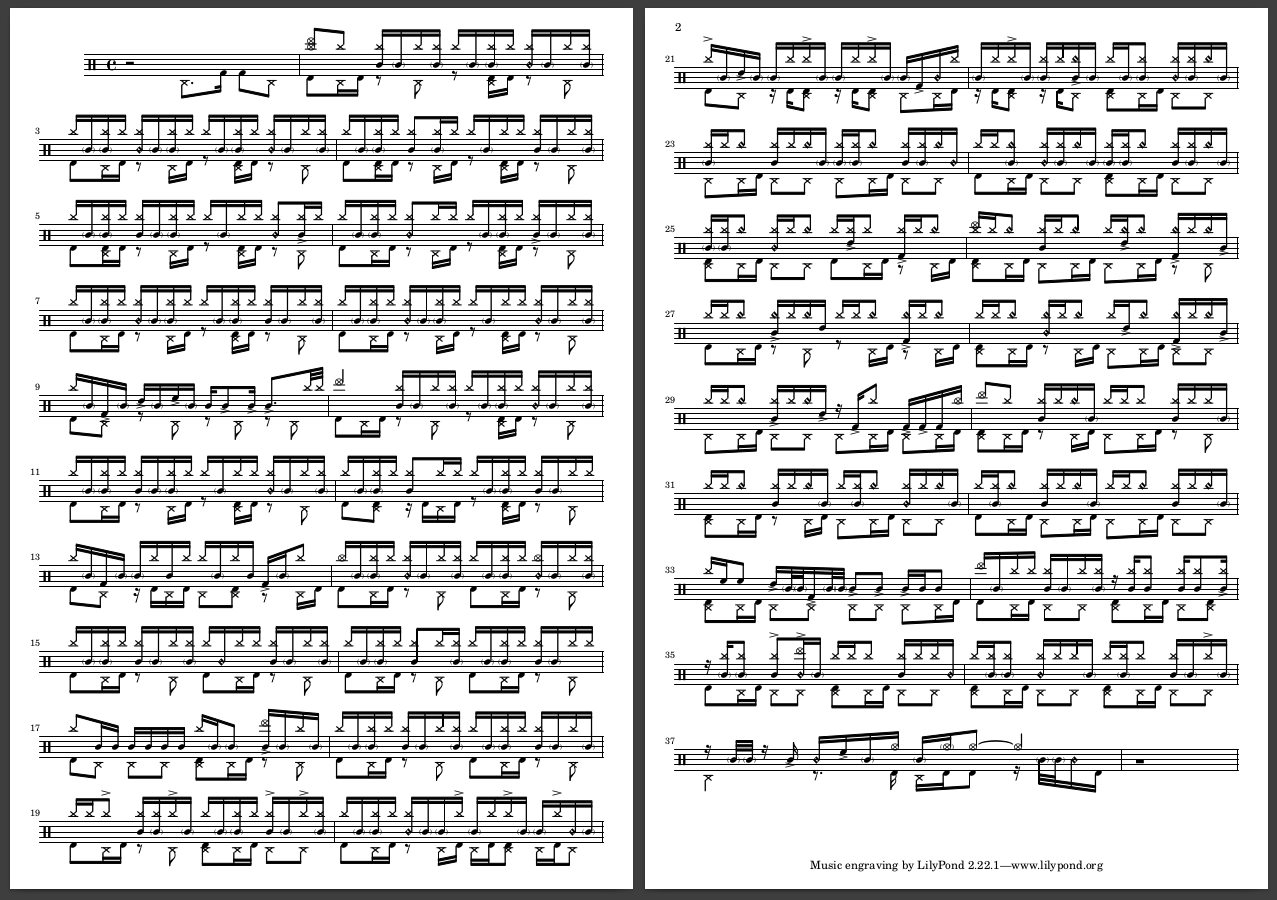
\includegraphics[height=120mm, width=160mm]{
    z_images/4_experimentations/1_analyses/3_partition.png}
    \caption{lilypond — transcription manuelle}
	\label{partition_ref}
\end{figure}

La partition de la figure \ref{partition_ref} est le résultat du code de la
figure \ref{extrait_code} (la totalité du code est mis en annexe et est
accessible sur le git). Cette partition a été totalement transcrite
manuellement avec lilypond par analyse des fichiers MIDI et audio
correspondants.

\begin{itemize}
    \item difficultés principales : trouver une application permettant de
        choisir librement la notation de la batterie. Lylipond le permet mais
        beaucoup de recherches ont été nécessaires pour comprendre l’ensemble
        des fonctionnalités permettant de faire fonctionner la notation
        « agostinienne » ainsi que les diverses subtilités de notations
        (accents, ghost-notes, flas, …).\\
        lylipond reste néanmoins un choix très agréable, une fois ces
        difficultés surmontées.
    \item Écrire la partition de la figure \ref{partition_ref} m’a pris
        beaucoup de temps car j’ai dû chercher comment écrire chaque nouvel
        évènement mais les autres transcriptions ont été beaucoup plus rapide
        et très aisées.
    \item Même si cela représente un investissement au départ, je recommande
        lylipond pour écrire la batterie et je pense que c’est meilleur outil
        pour cette tâche pour le moment. On peut configurer absolument tout.
    \item dans les autres logiciel d’édition de type musescore, la batterie
        est toujours confiné au système de notation américain.
    \item pour une comparaison entre système américain et système agostinien,
        voir section \ref{flas} est comparer les notations TM (agostinien) et
        TA (américain).
\end{itemize}


\section{Modélisation pour la transcription}
\label{modelisation_transcription}
\subsection*{Les pitchs}
\begin{table}[h]
	\centering
	\begin{tabular}{|c|c|c|} \hline
		Codes & Instruments & Pitchs \\ \hline
		cf & charley-main-fermé & 22, 42 \\
		co & charley-main-ouvert & 26 \\
		pf & charley-pied-fermé & 44 \\
		rd & ride & 51 \\
		rb & ride-cloche (bell) & 53 \\
		rc & ride-crash & 59 \\
		cr & crash & 55 \\
		cc & caisse claire & 38, 40 \\
		cs & cross-stick & 37 \\
		ta & tom-alto & 48, 50 \\
		tm & tom-medium & 45, 47 \\
		tb & tom-basse & 43, 58 \\
		gc & grosse caisse & 36 \\ \hline
	\end{tabular}
	\caption{Codes, identités et pitchs des instruments}
	\label{pitchs_instru}
\end{table}
Le tableau \ref{pitchs_instru} présente dans l’ordre, les codes des
instruments, leur identité (instrument ou parti d’un instrument — joué avec les
mains ou avec les pieds), le ou les pitchs qui lui sont associés.

Plusieurs pitchs peuvent parfois désigner le même instrument afin de pouvoir
supporter des kits de batterie plus larges (avec par exemple plusieurs toms
basses qui n’auraient pas tous exactement la même sonorité) ou simplement de
styles différents (pour chaque kits standard, ce sont les mêmes intruments mais
de styles différents)\footnote{Par exemple, les peaux des
toms jazz raisonnent alors que les toms rock sont mat.}.
J’ai regroupé les pitchs des différents types d’un même instrument dans une
seule ligne du tableau portant le nom du type de cet instrument. Ainsi,
plusieurs toms basses différents dans les données MIDI deviennent tous un tom
basse d’une batterie standard et la partition finale pourra être jouée sur
n’importe quel kit de batterie standard.

Malgré le large panel de pitchs disponibles, il semblerait qu’aucun pitch ne
désigne le charley ouvert joué au pied (« po » de la figure \ref{haut}).
Pourtant, dans la batterie moderne, plusieurs rythmes ne peuvent fournir le son
du charley ouvert qu’avec le pied car les mains jouent autre chose en même
temps. Cela doit en partie être dû à l’utilisation des boîtes à rythmes
en MAO qui ne nécessitent pas de faire des choix conditionnés par les
limitations humaines (2 pieds, 2 mains, et beaucoup plus d’instruments…)

\subsection*{La vélocité} \label{velocite}
La vélocité déterminera si les notes sont accentuées ou sont des ghost notes.
Pour les codes, je propose d’ajouter un suffix (« a » pour accent et «g» pour
ghost note) à la fin du code d’une note accentuée ou d’une ghost note.
Les choix pour déterminer si les notes sont accentuées ou sont des ghost notes
seront donnée dans la section \ref{partition_entiere}.

\subsection*{Les arbres de rythmes}
Les arbres de rythmes représentent un rythme dont les possibilités de notation
sur une partition sont théoriquement multiples. Les branchements sont des
divisions d’interval temporel, les feuilles sont des évènements musicaux
commençant au début de l’interval \cite{Laurson1996PatchWorkA}
\cite{Bresson_openmusicvisual} .\\
Voici une représentation qui fonctionne avec les 3 exemples de la figure
\ref{sep_voix} en arbre de rythmes avec les codes de chaque instrument :
\begin{figure}[h]
	\Tree[ [ [rd\\gc ][ [rd\\pf ][rd ]]]
	[ [rd\\cc ][ [rd\\pf ][rd ]]]
	[ [rd\\gc ][ [rd\\pf ][rd ]]]
	[ [rd\\cc ][ [rd\\pf ][rd ]]] ]
\end{figure}

Ci-dessous, le même arbre dont les codes des instruments sont remplacés par
leurs données MIDI respectives :
\begin{figure}[h]
	\Tree[ [ [51\\36 ][ [51\\44 ][51 ]]]
	[ [51\\38 ][ [51\\44 ][51 ]]]
	[ [51\\36 ][ [51\\44 ][51 ]]]
	[ [51\\38 ][ [51\\44 ][51 ]]] ]
\end{figure}

Chacun des trois exemples de la figure \ref{sep_voix} est représenté par un des
deux arbres syntaxiques ci-dessus.
<dam>complète un peu en précisant qu'on voit bien ici l'avantage des arbres
pour analyser ou construire la structure (les phrases ?) musicale</dam>

\section{Analyse syntaxique pour la transcription}

\begin{figure}[h]
\centering
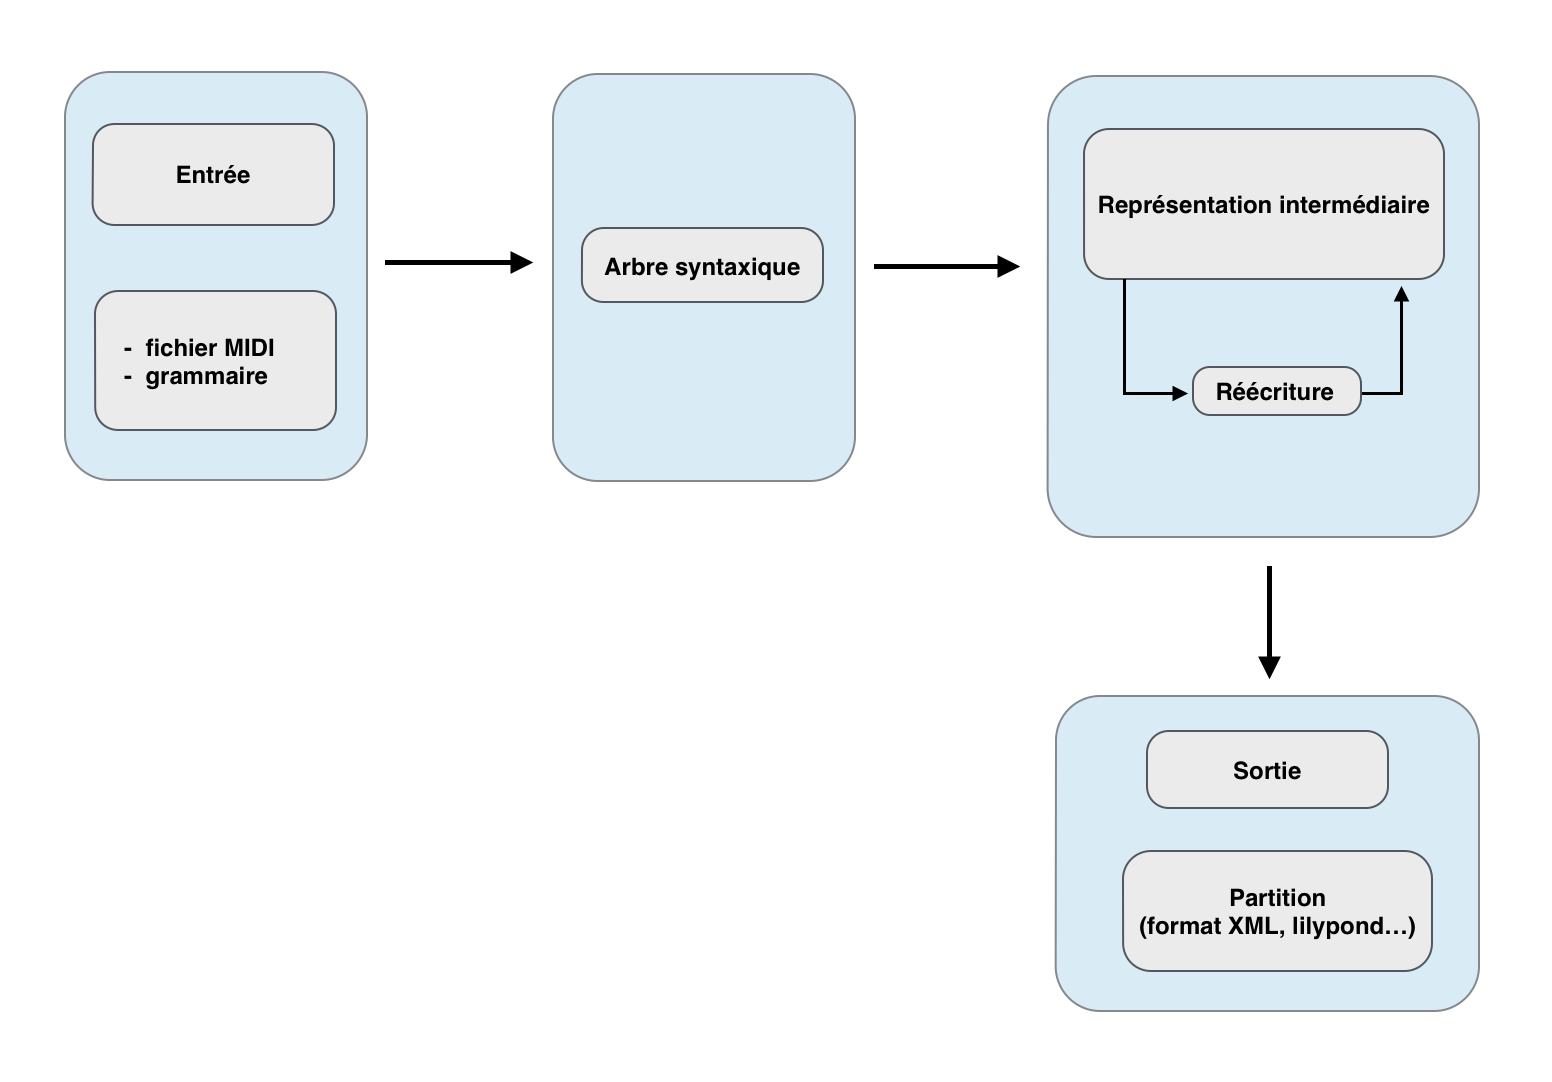
\includegraphics[height=70mm, width=110mm]{
z_images/3_methodes/1_Analyse_syntaxique/schema_qparse.png}
\caption{Présentation de Qparse}
\label{presentation_qparse}
\end{figure}

Comme le montre la figure \ref{presentation_qparse}, qparse\footnote{
\url{https://qparse.gitlabpages.inria.fr}} est un outil pour la transcription
musicale, qui, à partir d'une performance symbolique, séquentielle et non
quantifiée, produit une partition structurée. Il effectue conjointement des
tâches de quantification rhythmique et d'inférence de la structure de la
partition à l'aide de techniques d’analyse syntaxique (\textit{parsing}). Le
but du \textit{parsing} est en effet la structuration d'une représentation
séquentielle en entrée (un mot fini), suivant un modèle de langage
\cite{grune2007parsing}.

Dans le cas de qparse, le "mot" d'entrée est typiquement au format MIDI, et le
modèle de langage est une grammaire d'arbres pondérés représentant des
préférences en terme de notation musicale à produire \cite{droste2009handbook}.
basée sur des algorithmes d'analyse syntaxique pour les grammaires
arborescentes pondérées. En prenant en entrée une performance musicale
symbolique (séquence de notes avec dates et durées en temps réel, typiquement
un fichier MIDI), et une grammaire hors-contexte pondérée décrivant un langage
de rythmes préférés, il produit une partition musicale. Plusieurs formats de
sortie sont possibles, dont les formats XML (MEI, MusicXML,…), lilypond,…

Les principaux contributeurs sont :
\begin{itemize}
	\item Florent Jacquemard (Inria) : développeur principal.
	\item Francesco Foscarin (PhD, CNAM) : apprentissage ; Evaluation.
	\item Clement Poncelet (Salzburg U.) : integration de la librairie Midifile
        pour les input MIDI.
	\item Philippe Rigaux (CNAM) : production de partition au format MEI et de
        modèle intermédiaire de partition en sortie.
	\item Masahiko Sakai (Nagoya U.) : mesure de la distance input/output pour
        la quantification et CMake framework ; évaluation.
\end{itemize}

\subsection*{Les enjeux}
Plusieurs enjeux : <dam>idem à rédiger je suppose... un assez gros morceau
puisqu'il contiendra une partie de ta problématique appliquée</dam>
Le problème du MIDI avec Qparse\\
ON-OFF en entrée $\Rightarrow$ 1 seul symbole en sortie.\\
Minimiser la distance entre le midi et la représentation en arbre.\\
Un des problèmes de Qparse était qu’il était limité au monophonique.\\
Quelles sont les limites du monophonique ?\\
Impossibilité de traiter plusieurs voix et de reconnaître les accords.

\subsection*{La grammaire}
Il s’agit d’une grammaire hors-contexte pondérée…
<dam>incompréhensible ainsi, c'est dommage</dam>
// bar level\\
0 -> C0                1\\
0 -> E1                1\\
0 -> U4(1, 1, 1, 1)    1\\

// half bar level\\
9 -> C0                1\\
9 -> E1                1\\

// beat level\\
1 -> C0                1\\
1 -> E1                1\\
1 -> T2(2, 2)          1\\
1 -> T4(4, 4, 4, 4)    1\\

// croche level\\
2 -> C0                1\\
2 -> E1                1\\

// double level\\
4 -> C0                1\\
4 -> E1                1\\
4 -> E2                1\\
4 -> T2(6, 6)          1\\

// triple level\\
6 -> E1                1\\\\
Cette grammaire sépare les ligatures par temps au niveau de la mesure. Puis, au
niveau du temps, elle autorise les divisions par deux (croches) et par quatre
(doubles-croches). Tous les poids sont réglés sur 1. L’arbre de parsing en
résultant est considéré comme « convaincant » car il découpe correctement les
mesures et les temps.

\subsection*{Le parsing}
Les données MIDI sont quantifiées, les notes de dates proches sont alignées et
les relations entre les notes sont identifiées (accords, fla, etc…) ; un arbre
syntaxique global est créé ;

\subsection*{La représentation intermédiaire}
\begin{itemize}
    \item Les pitchs sont remplacés par les codes des instruments (voir tableau
    \ref{nom_instru_batt} ;
    \item réécriture 1 :\\
    séparation des voix $\Rightarrow$ un arbre par voix
    $\Rightarrow$ représentation intermédiaire (RI) ;
    \item réécriture 2 :\\
    simplification de l’écriture de chaque voix dans la RI.
    <dam>rédiger un peu mieux réécriture 1 et 2</dam>
\end{itemize}

\section{Les \textbf{formes rythmiques}}
\label{systemes_methodes}
Il existe en batterie des motifs rythmiques répétés (joués en boucle). Ces
motifs sont le résultat de la coordination de plusieurs instruments de la
batterie, je les nommerai \textbf{motifs} dans la suite du document. Très
souvent, un autre instrument est joué de manière indépendante sur le
\textbf{motif} mais en respectant la cohérence rythmique du \textbf{motif}. Je
nommerai \textbf{gamme} l’ensemble des combinaisons possibles pour cet autre
instrument. La \textbf{gamme} d’un \textbf{motif} est toujours relative à sa
signature rythmique. Enfin, j’ai nommé \textbf{forme rythmique} (\textbf{FR})
le couple \textbf{motif}-\textbf{gamme}.

\subsection*{Objectifs}
Le but est d'avoir des schemas types (les \textbf{formes rythmiques}) pour
calculer la séparation en voix. Cela constituerait une heuristique pour éviter
d'avoir à explorer une grande combinatoire.

Un ensemble de \textbf{formes rythmiques} comprenant leur signatures rythmiques
respectives et leurs règles spécifiques de réécriture sera nécessaire.

Une fois un système défini, la transcription à partir de l'entrée MIDI sera
facilitée par la reconnaissance de la FR qui contraindra le processus, il
premettra de :
\begin{itemize}
	\item définir une signature rythmique ;
	\item choisir une grammaire appropriée ;
	\item fournir les règles de réécriture (séparation des voix et
        simplification.
\end{itemize}

\subsection*{Définitions}

\begin{itemize}
    \item \textbf{motif} : rythmes coordonnés joués avec deux ou trois
        instruments coordonnés en boucle (répartis sur 1 ou 2 voix) ;
    \item \textbf{gamme} : Ensemble des combinaisons jouées par un autre
        instrument sur le \textbf{motif} (réparti sur 1 voix) ;
    \item \textbf{forme rythmique} : \textbf{motif} + \textbf{gamme}\\
\end{itemize}

Les \textbf{motifs} sont fixes, contrairement aux \textbf{gammes} regroupent
l’ensemble des possibilités qui peuvent être rencontrées en situation réelle
(sur une partition ou lors d’une performance de batterie).

Un \textbf{motif} détermine la signature rythmique d’une
\textbf{forme rythmique} , et donc de sa \textbf{gamme}. Il détermine aussi
avec quel instrument unique sera jouée la \textbf{gamme} et comment tous les
instruments de la \textbf{forme rythmique} se répartiront en voix.\\




Les \textbf{formes rythmiques} devront être distribuées dans 4 grandes
catégories\footnote{SR du tableau signifie « signature rythmique »}
\cite{system_drums} :
\begin{table}[h]
\centering
\begin{tabular}{|c|c|c|c|c|} \hline
\textbf{FR} & SR & Subdivisions & Possibles & nb
voix \\ \hline
binaires & simple & doubles-croches & triolets, sextolets & 2 \\
jazz & simple & triolets & croches et doubles & 2 \\
ternaires & complexe & croches & duolets, quartelets & 2 \\
afros-cubains & simple & croches & - & 3 \\ \hline
\end{tabular}
\caption{Sytèmes}
\end{table}\\
Nous exposerons 3 \textbf{formes rythmiques} afin d’illustrer les propos de
cette section :
\begin{itemize}
	\item 4/4 binaire 
	\item 4/4 jazz
	\item 4/4 afro-cubain
\end{itemize}

Le \textit{\textbf{motif}} et la

\subsubsection{Détection de la signature rythmique}
La partie \textbf{motif} des \textbf{FR} sera utilisée pour la
\textbf{définition des signature rythmiques}. 
La détection de la signature rythmique est importante, 
non seulement pour connaître le nombre de temps par mesure ainsi que le nombre
de subdivisions pour chacun de ces temps, mais aussi pour savoir comment écrire
l’unité de temps et ses subdivisions.

\begin{figure}[h]
	\centering
	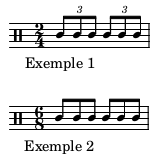
\includegraphics[height=40mm, width=40mm]{
    z_images/3_methodes/2_systemes/0_simple_VS_complexe.png}
	\caption{signature rythmique}
	\label{subdivisions}
\end{figure} %\newpage

La figure \ref{subdivisions} montre deux signatures rythmiques différentes. 
L’une (exemple 1) est \textit{simple} (2 temps binaires sur lesquels sont joués
des triolets), l’autre (exemple 2) est \textit{complexe} (2 temps ternaires). 
Le jazz est traditionnellement écrit en binaire avec ou sans triolet (même si
cette musique est dite ternaire alors que le rock ternaire sera plutôt écrit
comme dans l’exemple 2).

\subsubsection{Choix d’une grammaire}
Il faut prendre en compte l’existence potentielle de plusieurs grammaires
qui regroupent les contenus MIDI par signature rythmique. Le choix d’une
grammaire pondérée doit être fait avant le parsing puisque qparse prend en
entrée un fichier MIDI et un fichier wta (grammaire). C’est pour cette raison
que la signature rythmique doit être définie avant le choix de la grammaire.
Il faudrait les trouver automatiquement sans autres indications que les
contenus MIDI. Par conséquent, les \textbf{motifs} des
\textbf{formes rythmiques} devront être recherchés sur l’input (fichiers MIDI)
avant le lancement du parsing, afin de déterminer la signature rythmique en
amont. Cette tâche devra probablement être effectuée par utilisation
d'apprentissage automatique.


\subsubsection{Séparation des voix}

L’objectif de la procédure : ?

Le principe de la procédure : ?

Quelles sont les difficultés et les choix de séparation de voix et comment un
algorithme pourrait faire ces choix ?

\label{sys_sep_voix}
\begin{figure}[h]
	\centering
	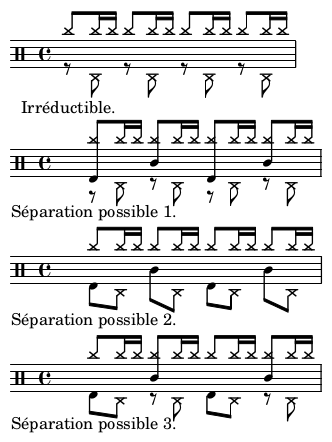
\includegraphics[height=60mm, width=40mm]{
    z_images/3_methodes/2_systemes/1_separation_4-4_binaire.png}
	\caption{\textbf{motif} 4-4 binaire}
	\label{binaire}
\end{figure}


Ici, la \textbf{forme rythmique} est construite sur un modèle rock avec une
signature rythmique en 4/4.

La première ligne de la figure \ref{binaire} est
appelée « Irréductible » car il n’y a pas d’autre choix de séparation des voix
pour la ride et le charley au pied.

La troisième séparation proposée est privilégiée car elle répartit selon deux 
voix, une voix pour les mains (ride et caisse claire) et une voix pour les
pieds (charley et grosse caisse). Ce choix paraît plus équilibré car deux
instruments sont utilisés par voix (contrairement séparations possibles 1 et 2
de la figure \ref{binaire}) et plus logique pour le lecteur puisque les mains
sont en haut et les pieds en bas.

\begin{figure}[h]
\centering
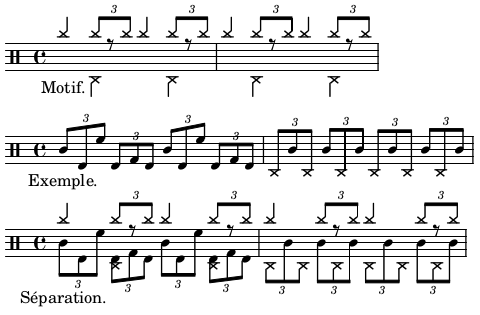
\includegraphics[height=45mm, width=60mm]{
z_images/3_methodes/2_systemes/2_separation_4-4_jazz.png}
\caption{\textbf{Motif} 4-4 jazz}
\label{jazz}
\end{figure}
\newpage
Dans la plupart des méthodes, le charley n’est pas écrit car il est considéré
comme évident en jazz traditionnel. Ici, le parti pris est de tout écrire.

Dans la figure \ref{jazz}, les mesures 1 et 2 de la ligne « Exemple » combinées
avec le \textbf{motif} de la première ligne, sont des cas typiques de la
batterie jazz. Tout mettre sur la voix haute serait surchargé. De plus, la
grosse caisse entre très souvent dans le flot des combinaisons de toms et de
caisse claire et son écriture séparée serait inutilement compliquée et peu
intuitive pour le lecteur. Le choix de séparation sera donc de laisser les
cymbales jouées à la main en haut, et les toms, la caisse claire, la grosse
caisse et la pédale de charley en bas.

\begin{figure}[h]
	\centering
	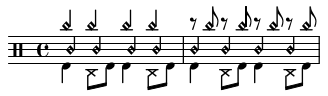
\includegraphics[height=20mm, width=70mm]{
    z_images/3_methodes/2_systemes/3_separation_afro-latins.png}
	\caption{\textbf{Forme rythmique} 4-4 afro-latin}
	\label{afro_latin}
\end{figure}

La figure \ref{afro_latin} montre un exemple minimaliste de
\textbf{forme rythmique} afro-latin \cite{system_drums}.

Cette \textbf{forme rythmique} doit être écrite sur trois voix car la voix
centrale est souvent plus complexe que sur la figure et la mélanger avec le
haut ou le bas serait surchargé et peu lisible.

\subsubsection{Simplification de l’écriture}

Les règles de \textbf{simplification} (les combinaisons de réécritures) seront
extraites des voix séparées des \textbf{formes rythmiques}.
Les explications qui suivent seront appuyées par une réécriture guidée dans la
section \ref{reecriture_guidee}.

Les \textbf{gammes} qui accompagnent les \textbf{motifs} étayent toutes les
combinaisons d’un \textbf{FR} et elles permettent, combinées avec le
\textbf{motif}, de définir ses propres règles de simplification.\\

Voici les différentes étapes à suivre :
\begin{itemize}
	\item pour chaque \textbf{gamme} d’une \textbf{forme rythmique}, faire un
        arbre de rythme représentant la \textbf{gamme} combinée avec le
        \textbf{motif} de la \textbf{FR} ;
	\item pour chaque arbre de rythmes obtenus, séparer les voix et faire un
        arbre de rythme par voix ;
	\item pour chaque voix (arbres de rythmes) obtenus, extraire tous les nœuds
        qui nécessitent une simplification et écrire la règle.\\
\end{itemize}

Certaines précisions concernant l’extraction de ces règles sont nécessaires. 
Il s’agit de précisions à propos de la durée, des silences et de la présence ou
non d’ouvertures de charley dans les instruments joués. 
Nous avons discuté de ces problèmes plus haut dans ce chapitre.\\

Voici quelques règles inhérentes à la simplication de l’écriture pour la
batterie :

Même si on favorise l’usage des silences pour l’écart entre les notes
n’appartenant pas au même temps, on les remplace systèmatiquement par un point
pour 2 notes au sein d’un même temps.

\begin{figure}[h]
	\centering
	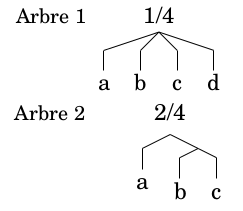
\includegraphics[height=45mm, width=50mm]{
    z_images/3_methodes/2_systemes/simplification_0.png}
	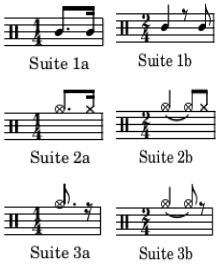
\includegraphics[height=50mm, width=40mm]{
    z_images/3_methodes/2_systemes/simplification_2.png}
	\caption{Simplifications — arbres et notations possibles}
	\label{simpl}
\end{figure}

Dans la figure \ref{simpl}, les « suites » sont des notations possibles
relatives aux arbres 1 ou 2.\\

\textit{Rappel :\\cf = charley fermé joué à la main ;\\co = charley ouvert joué
à la main ;\\ pf = charley fermé joué au pied.}\newpage

Soit l’arbre 1 de la figure \ref{simpl} dans lequel :
\begin{itemize}
    \item a et d sont des instruments de la batterie (x) ;
    \item b et c sont des continuations (t).
\end{itemize}
Pour chacune des conditions suivantes, une suite de la
figure \ref{simpl} est attribuée :
\begin{itemize}
	\item Si a n’est pas un co :\\
	$\Rightarrow$ Suite 1a.
	\item Si a est un co :
	\begin{itemize}
		\item Si d est un cf :\\
		$\Rightarrow$ Suite 2a.
		\item Si d est un pf :\\
		$\Rightarrow$ Suite 3a : d deviens un silence (r).\\
	\end{itemize}
\end{itemize}
Soit l’arbre 2 de la figure \ref{simpl} dans lequel :\\
a et c sont des instruments de la batterie (x) ;\\
b est une continuation (t) ;
Pour chacune des conditions suivantes, une suite de la figure \ref{simpl} est
attribuée :
\begin{itemize}
	\item Si a n’est pas un co :\\
	$\Rightarrow$ Suite 1b, b devient un silence.
	\item Si a est un co :
	\begin{itemize}
		\item Si c est un cf :\\
		$\Rightarrow$ Suite 2b, b devient une liaison et c devient un cf.
		\item Si c est un pf :\\
		$\Rightarrow$ Suite 3b : b deviens une liaison et c devient un silence.
	\end{itemize}
\end{itemize}

\section*{Conclusion}
Dans ce chapitre, nous avons formalisé une notation de la batterie inspirée des
méthodes de batterie Dante Agostini, modélisé cette notation pour
la transcription de données MIDI en partition.
Nous avons ensuite parlé de l’outil utilisé pour les transcriptions manuelles
en mettant en avant que cet outil devrait être utilisé pour la transcription de
la batterie et en précisant que tous les codes lilypond pour la création des
figures et partition de ce mémoire sont en accès libre sur github. Nous avons
ensuite décrit qparse qui l’outil que le travail de ce mémoire cherche à
améliorer.

Enfin, nous avons exposé une approche de type dictionnaire (les « formes
rythmiques ») pour détecter une signature rythmique, choisir une grammaire
pondérée appropriée et énoncer des règles de séparation des voix et de
simplification de l’écriture.


\chapter{Expérimentations}
\label{experimentations}
\minitoc
\section*{Introduction}
Dans ce chapitre, nous présenterons le jeu de données. Des analyses MIDI-Audio
seront effectuées sur ce jeu de données par le biais de comparaisons de
transcription et transcriptions manuelles avec lilypond. Nous aborderons aussi,
le passage du monophonique au polyphonique, indispensable pour l’application
des formes rythmiques dans la chaîne de traitement. Nous présenterons une
réécriture guidée par une forme rythmique qui devra être utilisé comme base de
connaissances pour augmenter la rapidité et la qualité en sortie de qparse et
comme une méthode de création de nouvelles formes rythmiques. Enfin, nous
discuterons sur l’ensemble des travaux finis, notamment les avancées réalisées
dans ce travail.

\section{Le jeu de données}
\label{gmd}
Nous avons utilisé le Groove MIDI
Dataset\footnote{\url{https://magenta.tensorflow.org/datasets/groove}}
\cite{groove2019} (GMD) qui est un jeu de données mis à disposition par Google
sous la licence Creative Commons Attribution 4.0 International (CC BY 4.0).\\
Le GMD est composé de 13,6 heures de batterie sous forme de fichiers MIDI et
audio alignés. Il contient 1150 fichiers MIDI et plus de 22 000 mesures de
batterie dans les styles les plus courants et avec différentes qualités de jeu.
Tout le contenu a été joué par des humains sur la batterie électronique Roland
TD-11 (figure \ref{electro_drums}).
\begin{figure}[h]
	\centering
	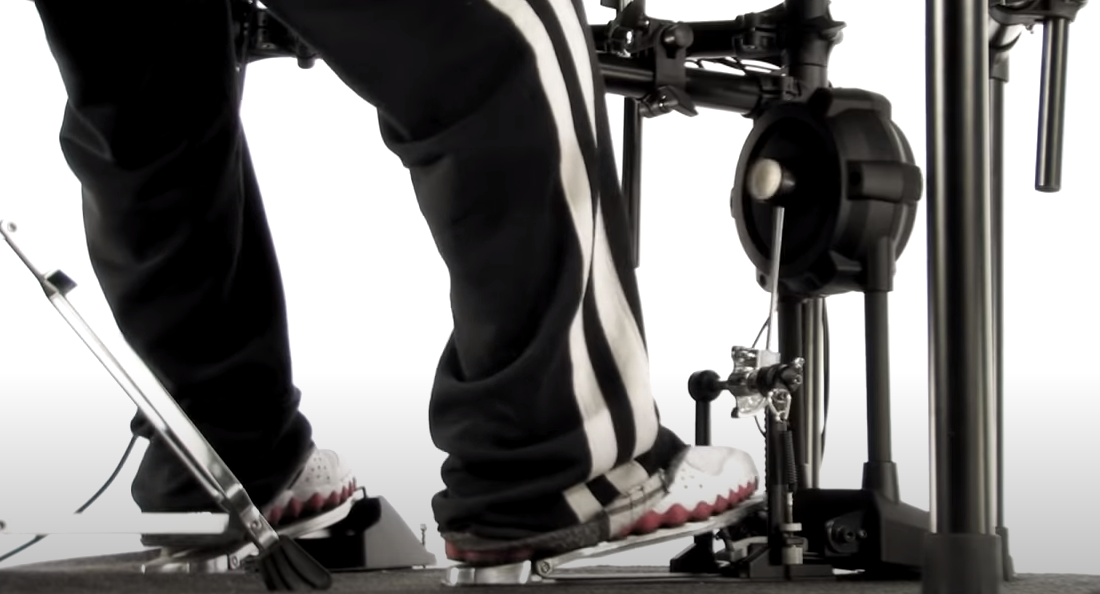
\includegraphics[height=35mm, width=60mm]
    {z_images/4_experimentations/0_groove/0_roland.png}\ \ 
	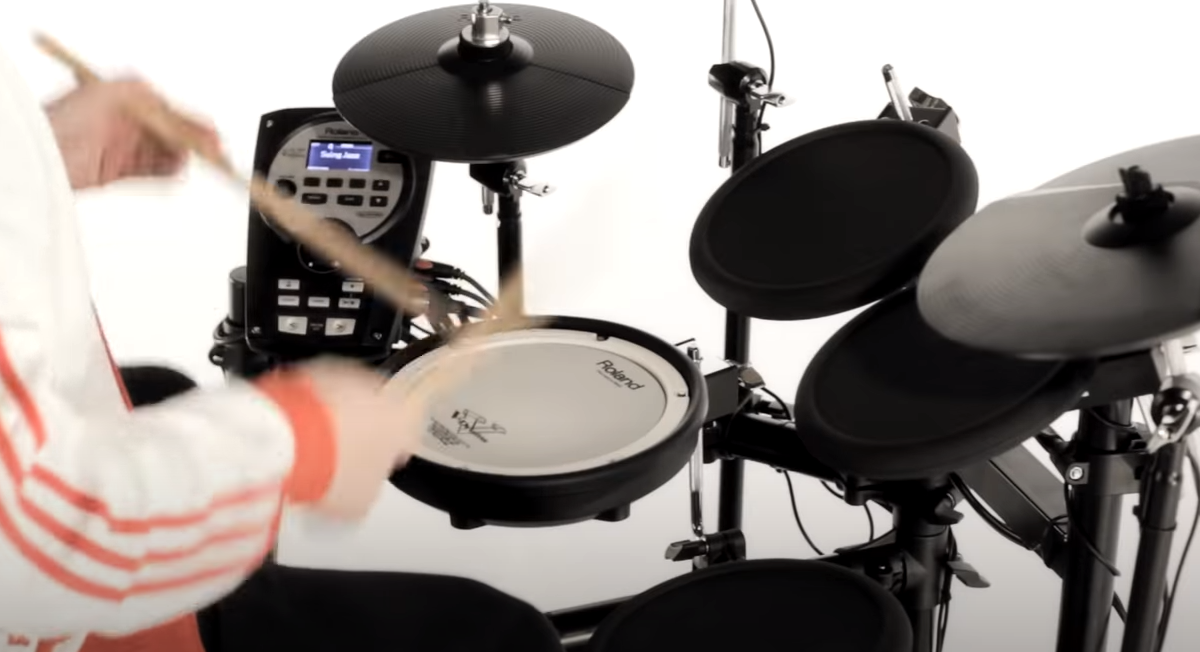
\includegraphics[height=35mm, width=60mm]
    {z_images/4_experimentations/0_groove/1_roland.png}
	\caption[Batterie électronique Roland TD-11]{Batterie électronique Roland
TD-11\footnotemark}
	\label{electro_drums}
	
\end{figure}
\footnotetext{\textit{Source~ :} \url{
    https://www.youtube.com/watch?v=BX1V_IE0g2c}}
Autres critères spécifiques au GMD~ :
\begin{itemize}
	\item Toutes les performances ont été jouées au métronome et à un tempo
        choisi par le batteur.
	\item 80\% de la durée du GMD a été joué par des batteurs professionnels
        qui ont pu improviser dans un large éventail de styles. Les données
        sont donc diversifiées en termes de styles et de qualités de jeu
        (professionnel ou amateur).
	\item Les batteurs avaient pour instruction de jouer des séquences de
        plusieurs minutes ainsi que des fills\footnote{Un \textit{fill} est une
        séquence de relance dont la durée dépasse rarement 2 mesures. Il est
        souvent joué à la fin d’un cycle pour annoncer le suivant.}.
	\item Chaque performance est annotée d’un style (fourni par le batteur),
        d’une signature rythmique et d’un tempo ainsi que d’une identification
        anonyme du batteur.
	\item Il a été demandé à 4 batteurs d’enregistrer le même groupe de 10
        rythmes dans leurs styles respectifs. Ils sont dans les dossiers
        eval-session du GMD.
	\item Les sorties audio synthétisées ont été alignées à 2 ms près sur leur
        fichier MIDI.
\end{itemize}

\subsection*{Format des données}
Le Roland TD-11 enregistre les données dans des fichiers MIDI et les divise en
plusieurs pistes distinctes~ :
\begin{itemize}
	\item une pour le tempo et l’indication de mesure~ ;
	\item une pour les changements de contrôle (position de la pédale de
        charley)~ ;
	\item une pour les notes.\\
\end{itemize}
Les changements de contrôle sont placés sur le canal 0 et les notes sur le
canal 9 (qui est le canal canonique pour la batterie).\\
Pour simplifier le traitement de ces données, ces trois pistes ont été
fusionnées en une seule piste qui a été mise sur le canal 9.

\section{Analyses et transcriptions manuelles}
\label{analyses_et_TM}
Ces analyses ont été faites dans le cadre de transcriptions manuelles à partir
de fichiers MIDI et Audio du GMD.

\subsection*{Comparaisons de transcriptions}
Pour les comparaisons de transcriptions, les transcriptions manuelles (TM) ont
été éditées à l’aide de Lilypond\footnote{\url{http://lilypond.org/}} ou
MuseScore\footnote{\url{https://musescore.com/}} et les transcriptions
automatiques (TA) ont toutes été générées par import d’un fichier MIDI dans
MuseScore.

\subsubsection{Exemple d’analyse 1}
\begin{figure}[h]
\centering
Transcription manuelle $\Rightarrow$ Transcription automatique
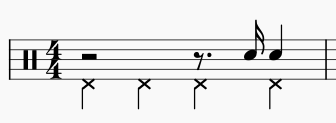
\includegraphics[height=20mm, width=50mm]{
z_images/4_experimentations/1_analyses/0_drummer1_session3/1_manuelle.png}
\ \ \ \ 
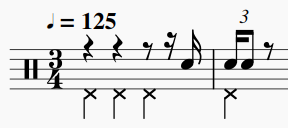
\includegraphics[height=20mm, width=45mm]{
z_images/4_experimentations/1_analyses/0_drummer1_session3/0_musescore.png}
\end{figure}
\begin{itemize}
	\item Erreur d’indication de mesure (3/4 au lieu de 4/4)~ ;
	\item Les silences de la mesure 1 de la TA sont inutilement surchargés~ ;
	\item La noire du temps 4 de la mesure 1 de la TM est devenue les deux
        premières notes (une double-croche et une croche) d’un triolet sur le
        temps 1 de la mesure 2 de la TA.
\end{itemize}

\subsubsection{Exemple d’analyse 2}
\begin{figure}[h]
\centering
\tab Transcription manuelle $\Rightarrow$ Transcription automatique\\
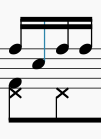
\includegraphics[height=20mm, width=13mm]{
z_images/4_experimentations/1_analyses/0_drummer1_session3/5_manuelle.png}
\ \ \ \ 
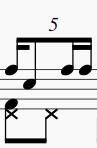
\includegraphics[height=20mm, width=13mm]{
z_images/4_experimentations/1_analyses/0_drummer1_session3/4_musescore.png}
\end{figure}
\begin{itemize}
	\item Les doubles croches ont été interprétées en quintolet
	\item La deuxième double-croche est devenue une croche.
\end{itemize}

\subsubsection{Exemple d’analyse 3}
\begin{figure}[h]
\centering
Transcription manuelle $\Rightarrow$ Transcription automatique
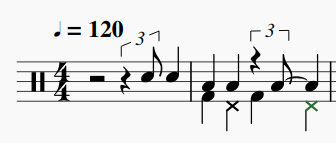
\includegraphics[height=24mm, width=50mm]{
z_images/4_experimentations/1_analyses/0_drummer1_session3/3_manuelle.png}
\ \ \ \ 
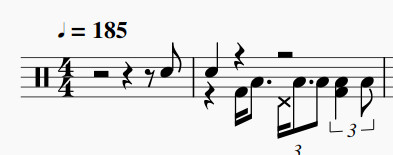
\includegraphics[height=25mm, width=55mm]{
z_images/4_experimentations/1_analyses/0_drummer1_session3/2_musescore.png}
\end{figure}

\begin{itemize}
	\item Les grosses-caisses, les charleys et les caisses-claires ont été
        décalés d’un temps vers la droite.
	\item Les toms basses des temps 1 et 2 de la mesure 2 de la TM ont été
        décalés d’une double croche vers la droite dans la TA.
	\item La première caisse claire de la mesure 1 devient binaire dans la TA
        alors qu’elle appartenait à un triolet dans la TM.
	\item Le triolet de tom-basse du temps 4 de la mesure 2 de la TA n’existe
        pas la TM.\\
\end{itemize}

\subsubsection{Exemple d’analyse 4}
\tab \tab Transcription manuelle $\Rightarrow$ Transcription automatique
\begin{figure}[h]
\centering
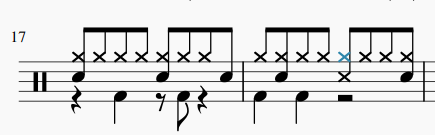
\includegraphics[height=19mm, width=50mm]{
z_images/4_experimentations/1_analyses/1_drummer1_session1/3_manuelle.png}
\ \ \ \ 
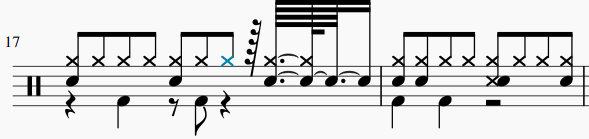
\includegraphics[height=19mm, width=70mm]{
z_images/4_experimentations/1_analyses/1_drummer1_session1/2_musescore.png}
\end{figure}

Sur le temps 4 de la mesure 1, la deuxième croche a été transcrite d’une
manière excessivement complexe!

\subsubsection{Exemple d’analyse 5 (flas)}
\label{flas}
Transcription manuelle\\
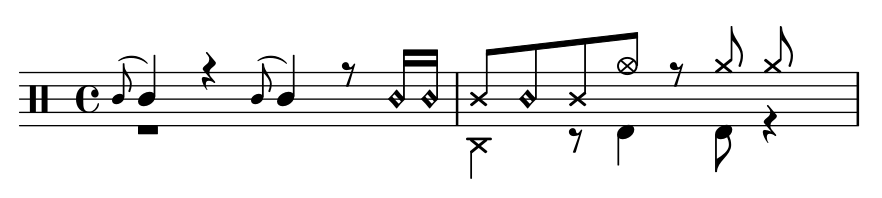
\includegraphics[height=25mm, width=95mm]{
z_images/4_experimentations/1_analyses/2_flas/0_124_funk_95_fill_4-4.png}\\
Transcription automatique\\\\
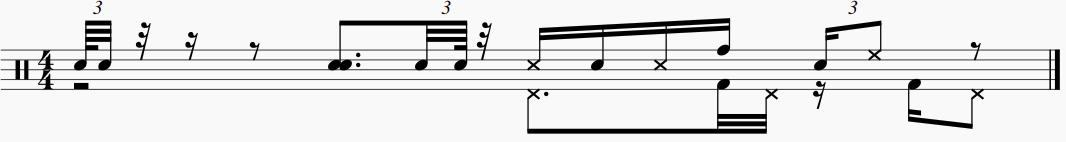
\includegraphics[height=20mm, width=130mm]{
z_images/4_experimentations/1_analyses/2_flas/1_124_funk_95_fill_4-4.png}\\

\begin{itemize}
	\item Le premier fla est reconnu comme étant un triolet contenant une
        quadruple croche suivie d’une triple croche au lieu d’une seule note
        ornementée.
	\item Le deuxième fla est reconnu comme étant un accord.
	\item Les deux double en contre-temps sur le temps 4 de la TM sont mal
        quantifiée dans la TA. 
	\item La TA ne reconnaît qu’une mesure quand la TM en transcrit deux. En
        effet, la TA a divisé par deux la durée des notes afin de les faire
        tenir dans une mesure à 4 temps dont les unités de temps sont les
        noires. Par exemple, le soupir du temps 2 de la TM devient un
        demi-soupir sur le contre-temps du temps 1 dans la TA. Ou encore, la
        noire (pf, voir le tableau \ref{pitchs_instru}) sur le temps 1 de la
        mesure 2 de la TM suivie d’un demi-soupir devient une croche pointée
        sur le temps 3 de la TA.
	\item Autre problème~ : certaines têtes de notes sont mal attribuées. Par
        exemple, le charley ouvert en contre-temps sur le temps 2 de la mesure
        2 de la TM devrait avoir le même symbole sur la TA. Idem pour les
        cross-sticks.
\end{itemize}

\subsubsection{Conclusion d’analyse}
Ces analyses ont montré la difficulté pour un logiciel comme MuseScore d’offrir
une partition lisible. Les raisons sont le fait que les fichiers MIDI ne sont
pas encore quantifiés mais aussi qu’il n’y a pas de reconnaissance de la forme 
du rythme impliquant sa position dans la mesure. Cette reconnaissance pourrait
permettre de rectifier les problèmes de signature rythmique ainsi que les
problèmes de décalage de temps. La reconnaissance de la forme du rythme
permettrait aussi de supprimer les aberrations du type de celle de l’exemple
d’analyse 4, puisque l’erreur sur cet exemple serait reconnue comme un élément
qui ne rentre pas dans le cadre de la forme de rythme en question. La dernière
raison qui rend le travail difficile est l’identification des flas, comment
savoir si deux notes jouées très proches sont~ :
\begin{itemize}
    \item séparées et rapides,
    \item mal jouées à l’unisson (accord),
    \item ou forment un fla ?
\end{itemize}


\subsection*{Transcription de partition}
\label{partition_entiere}
La figure \ref{partition_ref} est la transcription manuelle des fichiers
\textit{004\_jazz-funk\_116\_beat\_4-4.mid} et
\textit{004\_jazz-funk\_116\_beat\_4-4.wav} du GMD.

Cette transcription a été entièrement faite avec Lilypond (voir le code
lilypond sur le git \url{https://github.com/MartinDigard/Stage_M2_Inria}). Il
s’agit d’une partition d’un 4/4 binaire dont le fichier MIDI est annoncé dans
le GMD de style «~jazz-funk~» probablement en raison de la ride de type shabada
rapide (le ternaire devient binaire avec la vitesse) combiné avec l’after-beat
de type rock (caisse claire sur les deux et quatre).

La transcription manuelle de la partition de la figure \ref{partition_ref} et
l’analyse d’autre fichiers MIDI (voir section \ref{analyses_et_TM}) m’ont mené
aux observations suivantes~ :
\begin{itemize}
	\item Vélocité inférieure à 40~ : ghost-note.
	\item Vélocité supérieure à 90~ : accent.
	\item Pas d’intention d’accent ni de ghost-note pour une vélocité entre 40
        et 89.
	\item Les accents et les ghosts-notes ne sont significatifs ni pour les
        instruments joués au pied, ni pour les cymbales crash.\\
	En effet, certaines vélocités en dessous de 40 étant détectées et inscrites
    dans les données MIDI sont dues au mouvement du talon du batteur qui bat la
    pulsation sans particulièrement jouer le charley. Ce mouvement est perçu
    par le capteur de la batterie électronique mais le charley n’est pas joué.
	\item Au final, j’ai relevé les ghost-notes et les accents pour la caisse
        claire ainsi que les accents pour les toms et les cymbales rythmiques
        (charley et ride).
\end{itemize}


\subsubsection{Conclusion sur les transcriptions manuelles}
La transcription des données audio et MIDI contenues dans ces fichiers a permis
une analyse plus approndie des critères à relever pour chaque évènement MIDI et
de la manière de les considérer dans un objectif de transcription en partition
lisible pour un musicien (Voir la section \ref{modelisation_transcription}).


\section{Transcription polyphonique par parsing}
\label{jam}
Les Jams permettent de passer du monophonique au polyphonique.
On regroupe tous les évènements qu’on estime être à des dates suffisamment
proches dans des clusters que nous avons appelés «~Jam~».
Un Jam représente une séquence de points successifs dans un segment d’entrée
avec des informations supplémentaires sur leur rôle respectif, en supposant
qu’ils sont tous alignés à la même date lors de la quantification. Un Jam est
caractérisé par l’index de son premier point dans le segment d’entrée et sa
longueur (nombre de points).
Une fois dans les Jams, les évènements sont identifiés selon les critères
suivants~ :
\begin{itemize}
    \item \textit{Ignored}, les offsets sont ignorés~ ;
    \item \textit{Note}, si c’est une note simple~ ;
    \item \textit{Rest}, si c’est un silence~ ;
    \item \textit{GraceNote}, si c’est un fla~ ;
    \item \textit{Error}.
\end{itemize}

\section{Réécriture guidée par une forme rythmique}
\label{reecriture_guidee}
La démonstration qui suit est basée sur la partition de référence de la figure
\ref{partition_ref} puisque la forme rythmique qui sera utilisée en est
directement extraite.\\

Nous allons montrer~ :
\begin{itemize}
    \item la composition de cette forme rythmique~ ;
    \item son état final, c’est à dire toutes les combinaisons entièrement
        écrites en notation correcte sur partition~ ;

        $\Rightarrow$ cela constituera une référence pour la réécriture~ ;
    \item un exemple de transformation de la forme rythmique en arbre de
        rythme~ ;
    \item l’application de la séparation des voix sur cet exemple basé sur la
        référence citée précédemment (la forme rythmique en question)~ ;\\
        $\Rightarrow$ l’arbre de départ sera alors séparé en autant d’arbres
        qu’il y a de voix (deux arbres pour cette forme rythmique)~ ;
    \item les règles de simplification propres à la forme rythmique dont nous
        parlons. 
\end{itemize}
L’objectif de cette démonstration est de montrer comment un jeu de plusieurs
formes rythmiques pourrait être implémenté dans le cadre d’une approche
dictionnaire.

\subsection*{Motifs et gammes}
\begin{figure}[h]
\centering
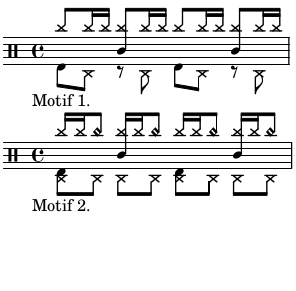
\includegraphics[height=43mm, width=40mm]{
z_images/4_experimentations/2_reecriture_guidee/0_motifs_4-4_binaires.png}
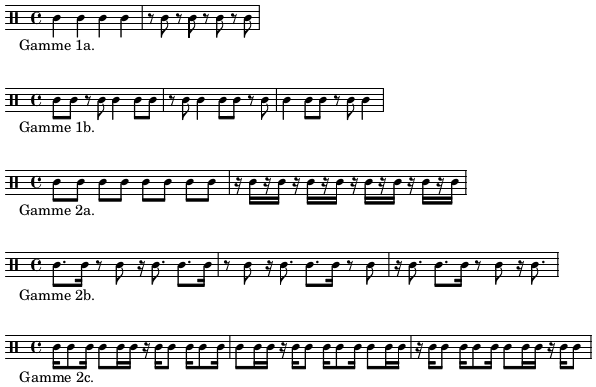
\includegraphics[height=55mm, width=85mm]{
z_images/4_experimentations/2_reecriture_guidee/1_gammes_4-4_binaires.png}
\caption{Motifs et gammes}
\label{motifs_gammes}
\end{figure}

\subsubsection{Motifs}
À partir de la partition de référence, les deux motifs de la figure
\ref{motifs_gammes} peuvent être systématisés. Le motif 1 est joué du début
jusqu’à la mesure 18 avec des variations et des fills et le motif 2 est joué de
la mesures 23 à la mesure 28 avec des variations. Ces deux motifs sont très
classiques et pourront être détectés dans de nombreuses performances.\\

\subsubsection{Gammes}
Les gammes de la figure \ref{motifs_gammes} étayent toutes les combinaisons
d’un motif en 4/4 binaires jusqu’aux doubles croches.\\
Les lignes 1 et 2 traitent les croches. La ligne 1 a 2 mesures dont la première
ne contient que des noires et la deuxième que des croches en contre-temps. Ces
deux possibilités sont combinées de manière circulaire dans les 3 mesures de la
deuxième ligne.\\
Les lignes 3, 4 et 5 traitent les doubles-croches. La ligne 3 a 2 mesures dont
la première ne contient que des croches et la deuxième que des doubles-croches
en contre-temps. Ces deux possibilités sont combinées de manière circulaire
dans les lignes 4 et 5 qui contiennent chacunes 3 mesures.

\subsection*{Formes rythmiques — motifs et gammes combinés}
Pour la suite de cette démonstration, j’utiliserai le motif 1 de la
figure \ref{motifs_gammes}.
\begin{figure}[h]
\centering
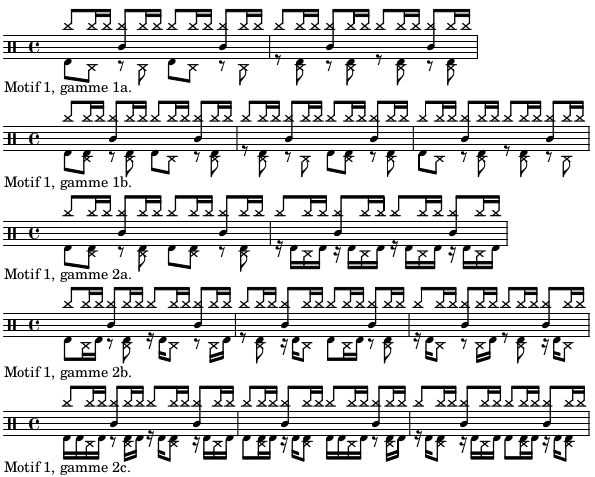
\includegraphics[height=75mm, width=85mm]{
z_images/4_experimentations/2_reecriture_guidee/2_systeme_4-4_binaire.png}
\caption{Partition d’un forme rythmique en 4/4 binaire}
\label{sys_binaire}
\end{figure}
\subsection*{Représentation de la forme rythmique en arbres de rythmes}
\label{demo_sys}
\begin{figure}[h]
	\centering
	\resizebox{350pt}{!} {
		\Tree[.Motif\ 1\ +\ gamme\ 1a
		[.Mesure\ 1
		[.Temps\ 1 [rd\\bd ][ [rd\\pf ][rd ]]]
		[.Temps\ 2 [rd\\cc ][ [rd\\pf ][rd ]]]
		[.Temps\ 3 [rd\\bd ][ [rd\\pf ][rd ]]]
		[.Temps\ 4 [rd\\cc ][ [rd\\pf ][rd ]]] ]
		[.Mesure\ 2
		[.Temps\ 1 [rd ][ [rd\\bd\\pf ][rd ]]]
		[.Temps\ 2 [rd\\cc ][ [rd\\bd\\pf ][rd ]]]
		[.Temps\ 3 [rd ][ [rd\\bd\\pf ][rd ]]]
		[.Temps\ 4 [rd\\cc ][ [rd\\bd\\pf ][rd ]]] ]]}
	\caption{Représentation arborescente d’une forme rythmique}
	\label{arbre_sys}
\end{figure}
L’arbre de la figure \ref{arbre_sys} servira de base pour le suite de
l’expérimentation. Comme indiqué à la racine de l’arbre, il représente la
première ligne de la figure \ref{sys_binaire}. Même si cet arbre représente
parfaitement le rythme concerné, il manque des indications de notation telles
que les voix spécifiques à chaque partie du rythme ainsi que les choix
d’écriture pour les distances qui séparent les notes de chaque voix entre elles
en termes de durée.

\subsection*{Réécriture — séparation des voix et simplification}
\subsubsection{La séparation des voix}
Ainsi l’arbre syntaxique de départ est divisé en autant d’instruments qui le
constituent et les voix sont regroupées en suivant les régles de la forme
rythmique.
\begin{figure}[h]
	\centering
	\resizebox{350pt}{!} {
		\Tree[.Motif\ 1\ +\ Gamme\ 1a
		[.Mesure\ 1
		[.Temps\ 1 [rd ][ [rd ][rd ]]]
		[.Temps\ 2 [rd\\cc ][ [rd ][rd ]]]
		[.Temps\ 3 [rd ][ [rd ][rd ]]]
		[.Temps\ 4 [rd\\cc ][ [rd ][rd ]]] ]
		[.Mesure\ 2
		[.Temps\ 1 [rd ][ [rd ][rd ]]]
		[.Temps\ 2 [rd\\cc ][ [rd ][rd ]]]
		[.Temps\ 3 [rd ][ [rd ][rd ]]]
		[.Temps\ 4 [rd\\cc ][ [rd ][rd ]]] ]]}
	\caption{arbre de rythmes — voix haute}
	\label{voix_haute}
\end{figure}\\
La voix haute (figure \ref{voix_haute}) regroupe la ride et la caisse claire
sur les ligatures du haut.
\begin{figure}[h]
	\centering
	\resizebox{350pt}{!} {
		\Tree[.Motif\ 1\ +\ Gamme\ 1a
		[.Mesure\ 1
		[.Temps\ 1 [bd ][ [pf ][t ]]]
		[.Temps\ 2 [t ][ [pf ][t ]]]
		[.Temps\ 3 [bd ][ [pf ][t ]]]
		[.Temps\ 4 [t ][ [pf ][t ]]] ]
		[.Mesure\ 2
		[.Temps\ 1 [t ][ [bd\\pf ][t ]]]
		[.Temps\ 2 [t ][ [bd\\pf ][t ]]]
		[.Temps\ 3 [t ][ [bd\\pf ][t ]]]
		[.Temps\ 4 [t ][ [bd\\pf ][t ]]] ]]}
	\caption{arbre de rythmes — voix basse}
	\label{voix_basse}
\end{figure}\\
La voix basse (figure \ref{voix_basse} regroupe la grosse caisse et le charley
au pied sur les ligatures du bas.
\subsubsection{Les règles de simplifications}
L’objectif des règles de simplifications est de réécrire les écarts de durée
qui séparent les notes d’une manière appropriée pour la batterie et qui soit la
plus simple possible. Les ligatures relient les notes d’un temps entre elles
afin de rendre la pulsation visuelle.\\\\
Pour les figures ci-dessous~ :
\begin{itemize}
	\item x = une note~ ;
	\item r = un silence~ ;
	\item t = une continuation (point ou liaison)
\end{itemize}
\begin{figure}[h]
	\centering
	\resizebox{50pt}{!} {
		\Tree[.1/4 [x ][ [x ][t ]] ]
	}\ \ \ \ \ $\Rightarrow$\ \ \ \ \
	\resizebox{30pt}{!} {
		\Tree[.1/4 [x ][x ] ]
	}\\
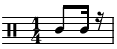
\includegraphics[height=10mm, width=25mm]{
z_images/4_experimentations/2_reecriture_guidee/simplification_0.png}\ \ \ \ \ 
$\Rightarrow$\ \ \ \ \
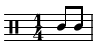
\includegraphics[height=10mm, width=20mm]{
z_images/4_experimentations/2_reecriture_guidee/simplification_1.png}
	\caption{Exemple de simplification 1}
	\label{1}
\end{figure}
\begin{figure}[h]
	\centering
	\resizebox{50pt}{!} {
		\Tree[.1/4 [t ][ [x ][t ]] ]
	}\ \ \ \ \ $\Rightarrow$\ \ \ \ \
	\resizebox{30pt}{!} {
		\Tree[.1/4 [r ][x ] ]
	}\\
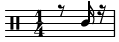
\includegraphics[height=10mm, width=25mm]{
z_images/4_experimentations/2_reecriture_guidee/simplification_2.png}\ \ \ \ \ 
$\Rightarrow$\ \ \ \ \
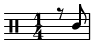
\includegraphics[height=10mm, width=20mm]{
z_images/4_experimentations/2_reecriture_guidee/simplification_3.png}
	\caption{Exemple de simplification 2}
	\label{2}
\end{figure}
\begin{figure}[h]
	\centering
	\resizebox{70pt}{!} {
		\Tree[.1/4 [x ][t ][x ][x ]]
	}\ \ \ \ \ $\Rightarrow$\ \ \ \ \
	\resizebox{50pt}{!} {
		\Tree[.1/4 [x ][ [x ][x ]]]
	}\\
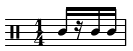
\includegraphics[height=10mm, width=25mm]{
z_images/4_experimentations/2_reecriture_guidee/simplification_4.png}\ \ \ \ \ 
$\Rightarrow$\ \ \ \ \
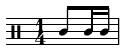
\includegraphics[height=10mm, width=20mm]{
z_images/4_experimentations/2_reecriture_guidee/simplification_5.png}
	\caption{Exemple de simplification 3}
	\label{3}
\end{figure}\newpage
\begin{figure}[h]
	\centering
	\resizebox{70pt}{!} {
		\Tree[.1/4 [t ][x ][x ][t ] ]
	}\ \ \ \ \ $\Rightarrow$\ \ \ \ \
	\resizebox{50pt}{!} {
		\Tree[.1/4 [ [r ][x ]][x ] ]
	}\\
\includegraphics[height=10mm, width=25mm]{
z_images/4_experimentations/2_reecriture_guidee/simplification_8.png}\ \ \ \ \ 
$\Rightarrow$\ \ \ \ \
\includegraphics[height=10mm, width=25mm]{
z_images/4_experimentations/2_reecriture_guidee/simplification_9.png}
	\caption{Exemple de simplification 4}
	\label{4}
\end{figure}
%\newpage
Ces règles ont été tirées de l’ensemble des arbres de la forme rythmique.

Les règles remplacent par un silence les continuations (t) qui sont au début
d’un temps. Cela est valable pour cette forme rythmique mais lorsqu’il y a des
ouvertures de charley, cela n’est pas toujours applicable.

\subsection*{Conclusion sur cette réécriture guidée}
La méthode des formes rythmiques étant basée sur une approche dictionnaire,
le premier objectif de cette réécriture guidée est d’orienter la recherche
d’autres formes rythmiques par observation du jeu de données et de montrer
comment les construire pour agrandir la base de connaissance de qparse pour la
transcription de la batterie.

\section{Discussion}

TRAVAUX EFFECTUÉS\\

Un système de formes rythmiques imposant chacune ses régles propres pour
l’écriture de partition de batterie a été formalisé. Une démonstration
théorique de ce système a permis de montrer comment créer des formes rythmiques
avec leurs régles propres
à partir de partition de référence pour agrandir le dictionnaire de formes
rythmiques. La théorie pour l’application de formes rythmiques sur un arbres
de parsing en \textit{input} de qparse pour appliquer les règles de réécriture
a été formalisé.\\ 

Il y a deux dimensions de le travail fourni~ :
\begin{enumerate}
    \item La volonté de pousser un exemple simple jusqu’au bout de la chaîne
        pour obtenir des résultats et une évaluation sur au moins un exemple~ ;
    \item La réalité du travail à fournir pour faire avancer sur la chaîne de
        traitement.
\end{enumerate}

Une solution aurait été de considérer les arbres de parsing obtenus après le
traitement du polyphonique comme un résultat local possible à évaluer au lieu
d’attendre que la chaîne arrive jusqu’à la génération d’une partition mais cela
n’était pas prioritaire pendant le stage.\\

Le choix de travailler avec lilypond au lieu de musescore a été pertinent car
il m’a permis d’établir une modélisation de la batterie avec une notation
cohérente accompagnée d’un fichier de configuration lilypond inspiré de la
notation Agostini et de nombreux exemples de scripts lilypond recouvrant
plusieurs phénomènes de notation en batterie utiles dans des contextes binaires
ou ternaires.\\

Nous avons améliorer le système de quantification de qparse pour la batterie,
notamment le passage à la polyphonie grâce aux Jams qui ont permis
l’identification des regroupements de note. En effet, avec la création de
grammaire adéquates, nous avons pu obtenir des arbres de parsing corrects en
sortie de qparse avec des exemples simples de fichiers MIDI.\\

TRAVAUX FUTURS\\
Le fait que lilypond utilise du texte (scripts) pour générer des partitions en
pdf pourrait permettre d’élaborer un système d’évaluation en utilisant la
comparaison de données textuelles. On pourrait par exemple, configurer
l’\textit{ouput} de qparse au format lilypond pour ensuite comparer une
partition de référence transcrite manuellement avec lilypond avec la sortie.
Comme il s’agit de comparer deux scripts, cette comparaison pourrait être
effectuée avec la commande «~diff~» .\\

Pour qu’une réelle évaluation soit possible, il faut que la chaîne de
traitement aille jusqu’à la génération d’une partition finale (après séparation
des voix et règles de réécriture). 
Matcher les motifs aurait été indispensable pour obtenir une quantité de
résultats qui justifieraient une évaluation automatique permettant de faire des
graphiques.\\


Il faudrait donc élaborer au moins suffisamment d’exemples pour que la
partition de référence soit entièrement générée afin de réaliser des
évaluations sur la sortie.\\

Création d’un jeu de forme rythmique basique réprésentatif des
        différents styles à recouvrir. Ce jeu n’a pas pu être créé, car comme
        vu plus haut, je me suis focalisé sur un exemple pour pouvoir le
        vérifier entièrement et dans l’espoir de pouvoir le tester en fin de
        chaîne.\\

SUITE\\

LLes formes rythmiques, qui constituent la proposition de ce mémoire,
nécessitent encore beaucoup de travail pour pouvoir être évaluées. Comme il
s’agit d’une approche dictionnaire, il faudrait créer beaucoup de formes
différentes avec chacune leur propres règles. L’objectif étant que cette
approche dictionnaire laisse la place à une génération de formes rythmiques en
apprentissage sur des données.

es formes rythmiques, qui constituent la proposition de ce mémoire,
nécessitent encore beaucoup de travail pour pouvoir être évaluées. Comme il
s’agit d’une approche dictionnaire, il faudrait créer beaucoup de formes
différentes avec chacune leur propres règles. L’objectif étant que cette
approche dictionnaire laisse la place à une génération de formes rythmiques en
apprentissage sur des données.



La transcription automatique de la batterie est un sujet passionnant mais
difficile~ : Obtenir la totalité des éléments nécessaires pour le mémoire
nécessiterait plus de temps. Une base solide spécifique à la batterie a
néanmoins été générée. Elle sera un bon point de départ pour les travaux futurs
dont plusieurs propositions sont énoncés dans le présent document.



\cleardoublepage\pdfbookmark[-1]{Conclusion générale}{conclusion}
\chapter*{Conclusion générale}
\adjustmtc
\addstarredchapter{Conclusion générale}
Dans ce mémoire, nous avons traité de la problématique de la transcription automatique de la batterie. Son objectif était de transcrire, à partir de leur représentation symbolique MIDI, des performances de batteur de différents niveaux et dans différents styles en partitions écrites.\\
Nous avons avancé sur le parsing des données MIDI établissant un processus de regroupement des évènements MIDI qui nous a permis de faire la transition du monophonique vers le polyphonique. Une des données importante de ce processus était de différencier les nature des notes d’un \textit{accord}, notamment de distinguer lorsque 2 notes constituent un \textit{accord} ou un \textit{fla}.\\
Nous avons établis des \textit{grammaires pondérées} pour le parsing qui correspondent respectivement à des métriques spécifiques. Celles-ci étant sélectionnables en amont du parsing, soit par indication des noms des fichiers MIDI, soit par reconnaissance de la métrique avec une approche dictionnaire de patterns prédéfinis \footnote{\textit{Motifs} dans les \textit{systèmes} de la présente proposition.} qu’il serait pertinent de mettre en œuvre en machine learning.\\
Nous avons démontré que l’usage des \textit{systèmes} élimine un grand nombre de calcul lors de la réécriture. Pour la séparation des voix grâce au motif d’un système et pour la simplification grâce aux gammes du motif d’un système. Nous avons aussi montré comment, dans des travaux futurs, un système dont le motif serait reconnu en amont dans un fichier MIDI pourrait prédéfinir le choix d’une grammaire par la reconnaissance d’une métrique et ainsi améliorer le parsing et accélérer les choix ultérieurs dans la chaîne de traitement en terme de réécriture.\\
Il sera également intéressant d'étudier comment l'utilisation de LM peut améliorer les résultats de l'AM, voir [2], et ouvrir la voie à la génération entièrement automatisée de partitions de batterie et au problème général de l'AMT de bout en bout.\cite{future_directions}


%%%%%%%%%%%%%%%%%%%%%%%%%%%%%%%%%%%%%%%%%%%%%%%%%%%%%%%%%%%%%%%%%%%%%%%%%%%%%%%%%%
\cleardoublepage\pdfbookmark[-1]{Bibliographie}{bibliography}
\bibliographystyle{unsrt}
\bibliography{x_biblio}
\appendix
\cleardoublepage\pdfbookmark[-1]{Annexes}{appendix}
\include{z_annexe_lilypond}
\cleardoublepage
\pdfbookmark[-1]{Index}{index}
\printindex
\end{document}
